%% For double-blind review submission, w/o CCS and ACM Reference (max submission space)
\documentclass[sigplan,10pt,review,anonymous]{acmart}
\settopmatter{printfolios=true,printccs=false,printacmref=false}
%% For double-blind review submission, w/ CCS and ACM Reference
%\documentclass[sigplan,review,anonymous]{acmart}\settopmatter{printfolios=true}
%% For single-blind review submission, w/o CCS and ACM Reference (max submission space)
%\documentclass[sigplan,review]{acmart}\settopmatter{printfolios=true,printccs=false,printacmref=false}
%% For single-blind review submission, w/ CCS and ACM Reference
%\documentclass[sigplan,review]{acmart}\settopmatter{printfolios=true}
%% For final camera-ready submission, w/ required CCS and ACM Reference
%\documentclass[sigplan]{acmart}\settopmatter{}


%% Conference information
%% Supplied to authors by publisher for camera-ready submission;
%% use defaults for review submission.
\acmConference[CC'20]{ACM SIGPLAN 2020 International Conference on Compiler Construction}{February 22--26, 2020}{San Diego, CA, USA}
\acmYear{2020}
\acmISBN{} % \acmISBN{978-x-xxxx-xxxx-x/YY/MM}
\acmDOI{} % \acmDOI{10.1145/nnnnnnn.nnnnnnn}
\startPage{1}

%% Copyright information
%% Supplied to authors (based on authors' rights management selection;
%% see authors.acm.org) by publisher for camera-ready submission;
%% use 'none' for review submission.
\setcopyright{none}
%\setcopyright{acmcopyright}
%\setcopyright{acmlicensed}
%\setcopyright{rightsretained}
%\copyrightyear{2018}           %% If different from \acmYear

%% Bibliography style
\bibliographystyle{ACM-Reference-Format}
%% Citation style
%\citestyle{acmauthoryear}  %% For author/year citations
%\citestyle{acmnumeric}     %% For numeric citations
%\setcitestyle{nosort}      %% With 'acmnumeric', to disable automatic
                            %% sorting of references within a single citation;
                            %% e.g., \cite{Smith99,Carpenter05,Baker12}
                            %% rendered as [14,5,2] rather than [2,5,14].
%\setcitesyle{nocompress}   %% With 'acmnumeric', to disable automatic
                            %% compression of sequential references within a
                            %% single citation;
                            %% e.g., \cite{Baker12,Baker14,Baker16}
                            %% rendered as [2,3,4] rather than [2-4].


%%%%%%%%%%%%%%%%%%%%%%%%%%%%%%%%%%%%%%%%%%%%%%%%%%%%%%%%%%%%%%%%%%%%%%
%% Note: Authors migrating a paper from traditional SIGPLAN
%% proceedings format to PACMPL format must update the
%% '\documentclass' and topmatter commands above; see
%% 'acmart-pacmpl-template.tex'.
%%%%%%%%%%%%%%%%%%%%%%%%%%%%%%%%%%%%%%%%%%%%%%%%%%%%%%%%%%%%%%%%%%%%%%


%% Some recommended packages.
\usepackage{booktabs}   %% For formal tables:
                        %% http://ctan.org/pkg/booktabs
\usepackage{subcaption} %% For complex figures with subfigures/subcaptions
                        %% http://ctan.org/pkg/subcaption

% packages
\usepackage{listings}
\usepackage{graphicx}
\usepackage{fancyhdr}
\usepackage{fancyvrb} % for Verbatim
\usepackage{hyperref}
\usepackage{color}
\usepackage{import}
\usepackage[ruled,vlined,noend]{algorithm2e} %see algorithm2e.pdf
\usepackage{url}
\usepackage[framemethod=TikZ]{mdframed}
%\usepackage{amsmath}
\usepackage{amsfonts} % for checkmark
\usepackage{multirow}
\usepackage{flexisym}
\usepackage{wrapfig}
\usepackage{tikz} % draw trees
\usepackage{epstopdf}
\usepackage{seqsplit}
\usepackage{graphics}

% For strike through of font - Joseph
\usepackage[normalem]{ulem}
%\usepackage{cancel}
%\usepackage{soul}
% For inparaenum environment. - Joseph
\usepackage{paralist}
\usepackage{comment}
\usepackage{setspace} % setstretch
\usepackage{svg}

% names
\newcommand{\addr}{School of Computer Science, McGill University, Montr\'eal, Canada}

% colors
\definecolor{Orange}{rgb}{1,0.5,0}
\definecolor{Blue}{RGB}{0,0,255}
\definecolor{OrangeRed}{RGB}{255,69,0}
\definecolor{LightGreen}{RGB}{11,83,69}
\definecolor{DarkYellow}{RGB}{160,64,0}
\definecolor{AntiqueBrass}{rgb}{0.8, 0.58, 0.46}
\definecolor{NiceBlue}{RGB}{11, 102, 163}
\definecolor{NiceRed}{RGB}{160, 64, 0}
\definecolor{Grey}{RGB}{128,128,128}
\definecolor{SlightRed}{RGB}{249,38,114}
\definecolor{SlightPink}{RGB}{155, 89, 182}

% I am using this color to highlight the text I am writing so that it is easy for you - Joseph
\definecolor{PineGreen}{rgb}{0.0, 0.47, 0.44}

\newcommand{\hgb}[1]{{\emph{\color{Blue}{#1}}}}
% \newcommand{\hgr}[1]{{\emph{\color{OrangeRed}{#1}}}}
\newcommand{\hgr}[1]{{\emph{\color{NiceRed}{#1}}}}
\newcommand{\hg}[1]{\emph{#1}}
\newcommand{\hglg}[1]{\emph{{\color{LightGreen}{#1}}}}
\newcommand{\hgdy}[1]{\emph{{\color{DarkYellow}{#1}}}}
\newcommand{\hga}[1]{\emph{{\color{AntiqueBrass}{#1}}}}

% tools
\newcommand{\todo}[1]{\hgb{Todo: #1}}
\newcommand{\joseph}[1]{\hglg{Joseph: #1}}
\newcommand{\hongji}[1]{\hgdy{Hongji: #1}}
\newcommand{\hanfeng}[1]{\hgr{Hanfeng: #1}}

% edit
\newcommand{\head}[1]{\vspace{1mm}\noindent\textbf{#1}\hspace{2mm}}
\newcommand{\headstep}[1]{\vspace{1mm}\noindent\textit{#1}\hspace{2mm}}
%\renewcommand{\baselinestretch}{1.2}
%\renewcommand{\lstlistingname}{Code} % update listing name's prefix

% ref
\newcommand{\refSec}[1]{Sec.~\ref{#1}}
\newcommand{\refFig}[1]{Fig.~\ref{#1}}
\newcommand{\refTable}[1]{Table~\ref{#1}}
\newcommand{\refListing}[1]{Listing~\ref{#1}}
\newcommand{\refAlgo}[1]{Algo.~\ref{#1}}
\newcommand{\refFoot}[1]{\footnote{\footnotesize{#1}}}

% syntax highlighting
\usepackage{textcomp} % other glyphs needed for upquote in listings below
\lstdefinelanguage{HorseIR}
{ basicstyle=\footnotesize\ttfamily,
  commentstyle=\color{Grey}\rmfamily\itshape,
  keywordstyle=\color{SlightPink},
  keywordstyle=[2]\color{NiceBlue},
  keywordstyle=[3]\color{NiceRed},
  keywordstyle=[4]\color{SlightRed},
  % list of keywords
  morekeywords={
  module,
  def,
  import
  },
  keywords=[2]{
  @table,
  @sum,
  @gt,
  @load_table,
  @column_value,
  @and,
  @compress,
  @enum,
  @list,
  @group,
  @values,
  @each_right,
  @raze,
  @compute_discount,
  @geq,
  @leq,
  @lt,
  @each,
  @len,
  @vector,
  @index_a,
  @index,
  @unique,
  @mul
  },
  keywords=[3]{
  table,
  sym,
  list,
  i64,
  f64,
  bool,
  },
  keywords=[4]{
  return,
  check_cast
  },
  sensitive=false, % keywords are not case-sensitive
  morecomment=[l]{//}, % l is for line comment
  morecomment=[s]{/*}{*/}, % s is for start and end delimiter
  morestring=[b]", % defines that strings are enclosed in double quotes
  upquote=true % ensures that backtick displays correctly
}

\usepackage[subtle]{savetrees}  %% three levels: subtle, moderate, extreme
%\usepackage{flushend} % has balanced columns on the last page
\usepackage{balance} % has balanced columns on the last page

%%%%%%%%%%%%%%%%%%%%%%%%%%%%%%%%%%%
%%% below for Damon 2019        %%%
%%%%%%%%%%%%%%%%%%%%%%%%%%%%%%%%%%%

\definecolor{mGreen}{rgb}{0,0.6,0}
\definecolor{mGray}{rgb}{0.5,0.5,0.5}
\definecolor{mPurple}{rgb}{0.58,0,0.82}
\definecolor{backgroundColour}{rgb}{0.95,0.95,0.92}

\lstdefinestyle{CStyle}{
   % backgroundcolor=\color{backgroundColour},   
   % commentstyle=\color{mGreen},
    commentstyle=\color{Grey}\rmfamily\itshape,
    %keywordstyle=\color{magenta},
    keywordstyle=\color{Blue},
    %numberstyle=\tiny\color{mGray},
    numberstyle=\color{mGray},
    stringstyle=\color{mPurple},
    %basicstyle=\footnotesize,
    basicstyle=\footnotesize\ttfamily,
    breakatwhitespace=false,         
    breaklines=true,                 
    captionpos=b,                    
    keepspaces=true,                 
    numbers=left,                    
    numbersep=5pt,                  
    showspaces=false,                
    showstringspaces=false,
    showtabs=false,                  
    tabsize=2,
    language=C,
    frame=single,
    xleftmargin=2mm,
    xrightmargin=2mm
}

\usepackage{xspace}
\usepackage{subcaption}

\newcommand{\scan}[2]{$\sigma$(#1, #2)}
\newcommand{\tuple}[6]{$\sum$(#1, #2, #3, #4, #5, #6)}
%\newcommand{\tupleSingle}[5]{$\sum$(#1, #2, #3, #4, #5)}
\newcommand{\TupleId}[2]{$\Gamma$(#1, #2)}
\newcommand{\TupleEOne}[1]{\TupleId{$E_1$}{#1}}
\newcommand{\TupleETwo}[1]{\TupleId{$E_2$}{#1}}
\newcommand{\TupleCase}[2]{$\Gamma\{$#1, #2$\}$}
\newcommand{\refTab}[1]{Table \ref{#1}}
\newcommand{\vv}{\vspace{3mm}}

\newcommand{\ruleFail}{\textit{NC}\xspace}  % NC = Not Conformable
\newcommand{\tupleNew}[3]{$\langle$#1, #2, #3$\rangle$}
\newcommand{\scanNew}[1]{$\sigma$(#1)}


\newcommand{\OldPaper}{\cite{Chen2018:HorseIR}\xspace}
\newcommand{\OldPaperAuthor}{Chen et al. \OldPaper}
\newcommand{\codeNCC}{\textit{NCC}\xspace}
\newcommand{\codeNCA}{\textit{NCA}\xspace}

\usetikzlibrary{shapes,snakes}


\lstdefinestyle{SQLStyle}{
   % backgroundcolor=\color{backgroundColour},   
    commentstyle=\color{mGreen},
    %keywordstyle=\color{magenta},
    keywordstyle=\color{mPurple},
    %numberstyle=\tiny\color{mGray},
    numberstyle=\color{mGray},
    %stringstyle=\color{mPurple},
    %basicstyle=\footnotesize,
    basicstyle=\footnotesize,
    breakatwhitespace=false,         
    breaklines=true,                 
    captionpos=b,                    
    keepspaces=true,                 
    numbers=left,                    
    numbersep=5pt,                  
    showspaces=false,                
    showstringspaces=false,
    showtabs=false,                  
    tabsize=2,
    language=sql,
    frame=single,
    xleftmargin=2mm
}

%%%%%%%%%%%%%%%%%%%%%%%%%%%%%%%%%%%
%%% below for CGO 20            %%%
%%%%%%%%%%%%%%%%%%%%%%%%%%%%%%%%%%%

\newcommand{\symbot}{$\bot$\xspace}
\newcommand{\symtop}{$\top$\xspace}
\newcommand{\symscan}[1]{$\sigma$(#1)}
\newcommand{\tupleSingle}[5]{\{(#1, #2, #3, #4, #5)\}}

\newcommand{\shapeS}{V(1)}
\newcommand{\shapeU}{U}
% \newcommand{\shapeVD}[1]{V$_d$(#1)}
% \newcommand{\shapeVC}[1]{V$_c$(#1)}
\newcommand{\shapeV}[1]{V(#1)}
\newcommand{\shapeVS}[1]{V$_s$(#1)}
\newcommand{\shapeN}{$I$}
\newcommand{\shapeE}{error}
\newcommand{\assign}{$\gets$}
\newcommand{\notok}{$\times$}
\newcommand{\pass}{\checkmark\xspace}

\newcommand{\shapeL}[2]{L(#1,#2)}
\newcommand{\rulesep}{\unskip\ \vrule\ } % add a vertical line between subfigure
\newcommand{\new}[1]{\emph{{\color{Blue}{#1}}}}
%\newcommand{\new}[1]{#1}

  % commonly used macros/imports/...

\begin{document}

\def\mytitle{Improving Database Query Performance with Automatic Fusion}
\def\mytitleinfo{\mytitle}

%% Title information
\title[\mytitleinfo]{\mytitle}          %% [Short Title] is optional;
                                        %% when present, will be used in
                                        %% header instead of Full Title.
%\titlenote{with title note}             %% \titlenote is optional;
                                        %% can be repeated if necessary;
                                        %% contents suppressed with 'anonymous'
%\subtitle{Subtitle}                     %% \subtitle is optional
%\subtitlenote{with subtitle note}       %% \subtitlenote is optional;
                                        %% can be repeated if necessary;
                                        %% contents suppressed with 'anonymous'


%% Author information
%% Contents and number of authors suppressed with 'anonymous'.
%% Each author should be introduced by \author, followed by
%% \authornote (optional), \orcid (optional), \affiliation, and \email.
%% An author may have multiple affiliations and/or emails; repeat the
%% appropriate command.
%% Many elements are not rendered, but should be provided for metadata
%% extraction tools.

\newcommand{\affil}{\affiliation{ \department{School of Computer Science} \institution{McGill University} }}

%% Author with single affiliation.
\author{Hanfeng Chen}
\affil
\email{hanfeng.chen@mail.mcgill.ca}

\author{Alexander Krolik}
\affil
\email{alexander.krolik@mail.mcgill.ca}

\author{Bettina Kemme}
\affil
\email{kemme@cs.mcgill.ca}

\author{Clark Verbrugge}
\affil
\email{clump@cs.mcgill.ca}

\author{Laurie Hendren}
\affil
\email{hendren@cs.mcgill.ca}
\orcid{0000-0001-6755-9632}

%\authornote{with author1 note}          %% \authornote is optional;
                                        %% can be repeated if necessary
%\orcid{nnnn-nnnn-nnnn-nnnn}             %% \orcid is optional
%\affiliation{
%  \position{Position1}
%  \department{Department1}              %% \department is recommended
%  \institution{Institution1}            %% \institution is required
%  \streetaddress{Street1 Address1}
%  \city{City1}
%  \state{State1}
%  \postcode{Post-Code1}
%  \country{Country1}                    %% \country is recommended
%}
%\email{first1.last1@inst1.edu}          %% \email is recommended

%% Author with two affiliations and emails.
%\author{Last2}
%\authornote{with author2 note}          %% \authornote is optional;
%                                        %% can be repeated if necessary
%\orcid{nnnn-nnnn-nnnn-nnnn}             %% \orcid is optional
%\affiliation{
%  \position{Position2a}
%  \department{Department2a}             %% \department is recommended
%  \institution{Institution2a}           %% \institution is required
%  \streetaddress{Street2a Address2a}
%  \city{City2a}
%  \state{State2a}
%  \postcode{Post-Code2a}
%  \country{Country2a}                   %% \country is recommended
%}
%\email{first2.last2@inst2a.com}         %% \email is recommended
%\affiliation{
%  \position{Position2b}
%  \department{Department2b}             %% \department is recommended
%  \institution{Institution2b}           %% \institution is required
%  \streetaddress{Street3b Address2b}
%  \city{City2b}
%  \state{State2b}
%  \postcode{Post-Code2b}
%  \country{Country2b}                   %% \country is recommended
%}
%\email{first2.last2@inst2b.org}         %% \email is recommended


%% Abstract
%% Note: \begin{abstract}...\end{abstract} environment must come
%% before \maketitle command


\begin{abstract}
With the development of column-based in-memory database systems the use of
array-based programming languages have shown to be promising for the execution
of database queries. In particular, they allow for an elegant representation of
query execution plans, that then can be further optimized using well
established techniques from compiler optimizations. However, it is not
straightforward to apply standard optimization techniques such as loop fusion
as database operators are best represented by advanced built-in functions that
can be quite complex. 
In this work, we apply a compiler approach to optimize SQL query execution
plans that are expressed in an array-based intermediate representation. We
analyze this code to determine shape properties of the data being
processed, and use a subsequent optimization phase to fuse multiple database
operators into single, compound operations, reducing the need for separate
computation and storage of intermediate values.  Experimental results on a
range of TPC-H queries show that our fusion technique is effective in
generating efficient code, improving query time over a baseline system.


%However, the database operators found in SQL queriessuch as loop fusion. They
%In this paper, we provide a systematic approach to apply loop fusion to
%array-based programming languages that are designed to support database
%queries. In-memory database systems (IMDBs) offer significant performance
%benefits to many applications in data analytics.
%With reduced I/O cost, however, good CPU performance is critical, but also
%difficult to achieve given the step-by-step nature of SQL execution.
%In this work we apply a compiler approach to optimize SQL queries in IMDBs.
%SQL execution plans are first translated to a custom, array-based intermediate
%representation.
%We analyze this code to determine shape properties of the data being processed,


% technique is effective in generating efficient code, improving query time by
% X\% over a baseline IMDB system.

\end{abstract}


%% 2012 ACM Computing Classification System (CSS) concepts
%% Generate at 'http://dl.acm.org/ccs/ccs.cfm'.
\begin{CCSXML}
<ccs2012>
<concept>
<concept_id>10011007.10011006.10011041</concept_id>
<concept_desc>Software and its engineering~Compilers</concept_desc>
<concept_significance>500</concept_significance>
</concept>
<concept>
<concept_id>10002951.10002952.10003190</concept_id>
<concept_desc>Information systems~Database query processing</concept_desc>
<concept_significance>500</concept_significance>
</concept>
</ccs2012>
\end{CCSXML}

\ccsdesc[500]{Software and its engineering~Compilers}
\ccsdesc[500]{Information systems~Database query processing}
%% End of generated code


%% Keywords
%% comma separated list
%\keywords{keyword1, keyword2, keyword3}  %% \keywords are mandatory in final camera-ready submission
\keywords{IR, Compiler optimizations, Array programming, SQL database queries, Loop fusion}


%% \maketitle
%% Note: \maketitle command must come after title commands, author
%% commands, abstract environment, Computing Classification System
%% environment and commands, and keywords command.
\maketitle

%   Budget (pages)
% ------------------
% Introduction   1.5
% Background     1   (+ Motivations)
% Optimizer      0.5
% Conf. Analysis 2.5
% Codegen        1.5
% Evaluation     2
% Related Work   0.5
% Con. + F.W.    0.5
% ------------------
% Total          10
%
% Budget goal: 10 pages with references excluded

\section{Introduction} \label{Sec:introduction}
While database systems have traditionally stored relational tables on a per-row
basis, recent developments have shown that a column-store format can outperform
traditional RDBMS for many workloads, particularly when the data fits into
main memory.
One of the first research prototypes of a column-based database manage systems
(DBMS) was MonetDB \cite{IdreosS2012}, still an active research project, but
many commercial systems now also support column-based storage (e.g.
Microsoft SQL Server~\cite{msqlserver},
SAP HANA~\cite{FarberF2012}, and
HyPer~\cite{Neumann2011:HyPer}).
% Microsoft SQL server
This fundamental shift in database architecture has resulted in a large body of
research efforts within the database community looking into efficient SQL query
execution on such a data format.

Given that in a column store each column of a table is stored as an array,
array programming languages appear as a promising construct to provide support
for query execution. In fact, \OldPaperAuthor introduced an intermediate
representation (IR) language, called \textit{HorseIR}, targeted at database
support.  SQL queries are first transformed into execution plans using
standard database optimization techniques that describe in which order and
how database operators such as joins, selections and aggregations should be
executed depending on the data to be analyzed. These execution plans are
then translated into HorseIR, the resulting code is optimized using
techniques from array programming, and finally the optimized code is
compiled into C code executable on different platforms.
% \OldPaper shows very good results on standard database benchmarks.

The approach used in HorseIR, however, does not take full advantage of the
optimization techniques available. Instead, it is restricted to basic code
fusion of element-wise operators, and although it explores some high-level
pattern-based optimization techniques, these require considerable knowledge of
database operators.  Optimization potential is also reduced by extensive use of
built-in functions, the complexity of which limits optimization.

For example, it is common for SQL queries to do a selection (selecting some
rows based on the filter criteria on one column) and then perform aggregation,
such as a summation.  In an array-based language this can be represented as

\begin{small}
\begin{Verbatim}[xleftmargin=.3\columnwidth]
R = sum(filter(C, A))
\end{Verbatim}
\end{small}

%%% $$
%%% R = sum(filter(C, A))
%%% $$

\noindent{}where the condition \texttt{C} is a boolean vector, the input array \texttt{A}
is a vector with the same number of elements, and the result \texttt{R} is a
scalar.  A straightforward way to generate C code from this is to generate two loops, the first applying the boolean selection and producing an intermediate result, and the second loop performing the reduction on this intermediate result.  A more optimized version, however, would fuse the two loops into one, performing the reduction on the fly and avoiding generation of an intermediate result:

\begin{center}
\begin{minipage}{\linewidth}
\begin{small}
\begin{lstlisting}[language=C, frame=single, xleftmargin=0mm, xrightmargin=5mm]
R=0;
for(int i=0; i<C.size; i++) {
    if(C[i]) { R += A[i]; } // true block
}
\end{lstlisting}
\end{small}
\end{minipage}
\end{center}

% add lines around box: frame=single
%\begin{small}
%\begin{Verbatim}[xleftmargin=.15\columnwidth]
%R=0;
%for(int i=0; i<C.size; i++) {
%    if(C[i]) { // true block
%        R += A[i];
%    }
%}
%\end{Verbatim}
%\end{small}

%%% \begin{lstlisting}[style=CStyle]
%%% for(int i=0; i<10; i++){
%%%     if(C[i]) { // true block
%%%         R += A[i]
%%%     }
%%% }
%%% \end{lstlisting}

%% However, HorseIR describes both sum and filter as built-in functions, and
%% currently no optimization across those functions can be performed.
\noindent{}The analysis required to generate such code from a series of built-in functions, however, is complex,
depending on non-trivial array dependency analysis as well as knowledge of array dimensions, and 
while possible in principle, our experience has been that these optimization opportunities are not found by our available C compilers.

% \refFig{fig:fusion_idea} shows that we propose automatic fusion which contains
% element-wise fusion and some parts of pattern-based fusion
% so that less pattern-based fusion is required.

\begin{figure}[htbp]
\centering
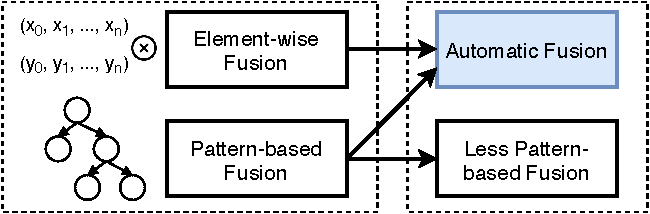
\includegraphics[width=.95\columnwidth]{./src/figure/basic-idea.pdf}
\caption{Introducing automatic fusion to optimize the array-based code
(HorseIR) generated from database queries with less pattern-based fusion.}
\label{fig:fusion_idea}
\end{figure}

In this paper we provide a more systematic approach to analyzing the query
program and generating optimized code.
As depicted in \refFig{fig:fusion_idea}, it is called \textit{automatic fusion}
which contains element-wise fusion and some parts of pattern-based fusion so
that less pattern-based fusion is required.
In particular, we provide a detailed analysis of the most important built-in
functions that are useful for executing SQL operators, and how we can optimize
across such functions.
To do so, we have a closer look at \textit{shape analysis}, and how shape propagates
when functions are combined. This allows us to use loop fusion extensively to
avoid unnecessary iterations over the data and intermediate results.  


% contribution
The contributions of this paper are summarized as follows:

\begin{itemize}
\item We explore a new approach to improve database query performance by
      applying techniques derived from array programming. We focus on HorseIR, an IR specifically designed to support database query execution.
\item We perform shape analysis on the built-in functions of HorseIR that represent database operators. This allows us to collect precise shape information and provide a conformability analysis to identify fusible sections in the HorseIR code. 
\item We present a set of optimization and code generation strategies to automatically
      generate optimized code.
\item We conduct experiments on the database benchmark TPC-H, to show the effectiveness of our technique.
\end{itemize}

\begin{comment}
The rest of this paper is organized as follows:
\refSec{Sec:background}
provides the background of HorseIR and array-based optimizations.
\refSec{Sec:overview}
introduces the description of the overview of our approach.
\refSec{Sec:shape}
presents our shape analysis for different groups of functions.
\refSec{Sec:conformability}
introduces our conformability analysis to identify fusible sections.
\refSec{Sec:codegen}
describes our code generation rules for generating efficient code.
\refSec{Sec:evaluation}
shows our experiments and experimental results.
\refSec{Sec:relatedwork}
discusses related work, and
\refSec{Sec:conclusion}
concludes.
\end{comment}


\section{Motivation and Background} \label{Sec:background}
% \hanfeng{Working on this section.  Please come back later!}

In this section, we first present the principles of loop fusion techniques for
array-based optimization, and then provide background on HorseIR and its
optimization capabilities. 

\subsection{Loop Fusion}

Loop fusion is an effective technique to improve program performance as
loops usually dominate the execution.
In the context of array-based languages, loop fusion is applied during the code
generation phase, when array-based functions are translated into loops of the
target language, e.g., C. The goal of loop fusion is to minimize the number of
loops in the target program.
There are two kinds of loop fusion as follows.

1. \textit{Fusion for removing intermediate results.}
For example, assume the sequence of two element-wise functions
\texttt{T = A*B, R = T+C}, where T, A, B, R, C are vectors of the same length
with no memory overlap.
A naive code-generation would translate this line-by-line into two loops for
the two arithmetic functions, first multiplication, then addition, with an
intermediate result vector T.
However, the element-wise functions can be easily fused generating a single
loop without intermediate vector (i.e., with loop body \texttt{R[i]=A[i]*B[i]+C[i]}).

2. \textit{Fusion when sharing the same loop head.}
Generally, when two loops share the same loop head (but have different loop
body), they often can be fused into a single loop in order to reduce the
overhead of iterating over the two loops individually. However, the bodies of
the two loops might have dependencies that make such a merge impossible. 

%%% \begin{lstlisting}[style=CStyle]
%%% // temp[10]: a temporary array
%%% for(int i=0; i<10; i++){
%%%         temp[i] = C[i] * D[i];
%%% }
%%% for(int i=0; i<10; i++){
%%%         A[i] = B[i] + temp[i];
%%% }
%%% \end{lstlisting}

%%% \begin{lstlisting}[style=CStyle]
%%% for(int i=0; i<10; i++){
%%%         A[i] = B[i] + C[i] * D[i];
%%% }
%%% \end{lstlisting}

%%% \todo{Explain how challenging loop fusion is.}

Ideally, a smart compiler can optimize loops in steps:
(1) resolve the data dependency between variables inside loops;
(2) identify the use of temporary, intermediate result arrays; and
(3) fuse the for loops and avoid the intermediate result arrays whenever possible.

However, automatic loop fusion is challenging for
compilers~\cite{Kennedy01:FastFusion,Kennedy1993:LoopFusion}.
Instead, we believe it is much easier if the potential of loop fusion is
already performed looking at the high-level language
(i.e., in the array-based program) due to the higher level of abstraction.

\subsection{HorseIR: an Array-based IR for SQL Queries}

HorseIR \OldPaper was designed to represent execution plans for SQL queries
where data is represented in column-format and assumed to reside in
main-memory. HorseIR represents the columns of the database tables as vectors,
and uses lists for compound data. It provides dozens of data types to
accommodate the many data types found in database systems. Moreover, it supports a
large set of array-based built-in functions that  represent the arithmetic and
database-related operators that are commonly used in SQL queries.

Fig.~\ref{fig:motivation_example} shows a motivating example of queries
executing with HorseIR framework. Fig.~\ref{fig:motivation_sql} shows a SQL
query on the database table \texttt{store\_items}. The WHERE clause represents
a selection filtering only those records of the table that fulfill certain
conditions on the \texttt{item_date} column. The SELECT clause projects on
columns \texttt{item_price} and \texttt{item\_discount}, performing an
element-wise arithmetic function (multiplication) and then aggregation over the
result. 

% http://www.texample.net/tikz/examples/simple-flow-chart/
\tikzstyle{line}  = [draw, ->, >=stealth]
\tikzstyle{block} = [node distance=8mm]

\begin{figure*}[htbp]

\begin{subfigure}[b]{.6\columnwidth}
\begin{lstlisting}[style=SQLStyle, basicstyle=\footnotesize]
SELECT
  SUM(item_price * item_discount) AS saving
FROM
  store_items
WHERE
  item_date > 2010.09.01 AND
  item_date < 2010.09.30;
\end{lstlisting}
\caption{An SQL query example} \label{fig:motivation_sql}
\end{subfigure}
\hfill
\begin{subfigure}[b]{.7\columnwidth}
\begin{lstlisting}[language=HorseIR, basicstyle=\footnotesize, literate = {-}{-}1]
// ... load columns from table
(S0) t0:bool = @gt(c0,2010-09-01:date);
(S1) t1:bool = @lt(c0,2010-09-30:date);
(S2) t2:bool = @and(t0, t1);
(S3) t3:f64  = @compress(t2, c1);
(S4) t4:f64  = @compress(t2, c2);
(S5) t5:f64  = @mul(t3, t4);
(S6) t6:f64  = @sum(t5);
// ... return result as a table
\end{lstlisting}
\caption{Core part of HorseIR code for (a) } \label{fig:motivation_horseir}
\end{subfigure}
% \hfill
\hspace{0.07\columnwidth}
\begin{subfigure}[b]{.6\columnwidth}
\centering
% xleftmargin=.15\columnwidth
\begin{lstlisting}[style=CStyle, basicstyle=\footnotesize]
//... load columns c0,c1,c2
t6 = 0;
for(int i=0; i<n; i++){
  if(c0[i] > 20100901
     && c0[i] < 20100930){
    t6 += c1[i] * c2[i];
  }
}
//... return t6, a scalar
\end{lstlisting}
\caption{Optimized C Code generated from (b)} \label{fig:motivation_c}
\end{subfigure}
\caption{Translating an SQL query from (a) to the corresponding HorseIR code shown in (b) (with columns: c0 (item_date), c1 (item_price), and c2 (item_discount)), and generating optimized C code in (c).} \label{fig:motivation_example}
\end{figure*}


Such a query is first translated into a query execution plan. The previous
work~\OldPaper uses the advanced query optimizer of the HyPer database
system~\cite{Neumann2011:HyPer} to generate high-performance execution plans.
Then, the execution plan is translated into HorseIR using both standard array
language and database-specific built-in functions. By not directly translating
queries into HorseIR but instead translating the optimized execution plans, the
approach leverages the extensive SQL-specific query optimization experience of
the database community.

Fig.~\ref{fig:motivation_horseir} shows the resulting HorseIR program without
optimization and many intermediate results. From there, the previous
work~\OldPaper proposes optimizations based on element-wise fusion and fusion
with patterns. For example, (S0) and (S1) in the HorseIR program are easily
fused into one statement, as \texttt{@gt} and \texttt{@lt} are element-wise
functions. Since there is a large set of such functions, this approach has
shown to be very beneficial. 
Moreover, generating parallel code for element-wise functions is easy as they
are dependence-free.


However, once functions are more complex, such as the \texttt{@compress}
functions of lines (S3) and (S4) in the example, fusion is no longer
straightforward, as these high-level built-in functions contain data-dependent
loops implicitly. 
Thus, fusion across such functions is not supported by the previous
work~\OldPaper which instead generates separate loops for them.
This can become a severe performance bottleneck, especially when the
intermediate results are barely reused. 

The boolean selection function \texttt{@compress} is common in SQL queries
because of the WHERE clause.
In the example, \texttt{t2} is a boolean vector indicating the indices of the
records that fulfill the filtering condition of the query. In (S3) and (S4)
@compress retrieves the corresponding element values of the
\texttt{item\_price} and \texttt{item\_discount} columns.
However, the intermediate results of \texttt{t3} and \texttt{t4} can be avoided
because the retrieval can be fused with the subsequent arithmetic and
aggregation functions. In fact, for the given example, it is possible to fuse and
generate a single loop as shown in Fig.~\ref{fig:motivation_example} (c).

In this paper, we show how fusion \textit{across} built-in functions can be
done automatically and systematically by using a principled shape and
conformability analysis. Importantly, although previous work~\OldPaper also fuses
operations, it is based on simplistic element-wise fusion and pattern rules. Using
patterns is quite challenging as it requires the expertise of SQL execution plans.
Furthermore, there exist many different types of queries, and thus potentially many
different patterns. It is not clear, whether the patterns presented in \OldPaper are
exhaustive. 

\section{Overall Structure of the Optimizer} \label{Sec:overview}
\begin{figure}[htbp]
\centering
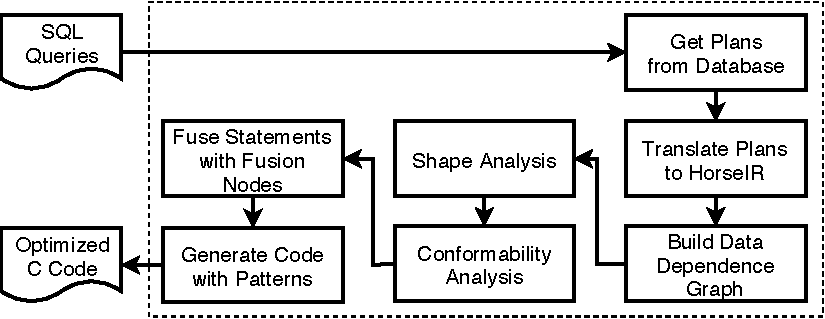
\includegraphics[width=\columnwidth]{./src/figure/overview-v4.pdf}
\caption{Analysis and code generation overview.} \label{fig:overview}
\end{figure}

We have implemented our approach for generating fused and efficient
\texttt{C} code in the HorseIR compiler. An overview of the workflow
can be found in \refFig{fig:overview}.

Just as in previous work~\OldPaper, we first generate an optimized
query execution plan using the HyPer database system~\cite{Neumann2011:HyPer}
\footnote{We can access HyPer's plan generator online, but HyPer's execution
engine is not publicly available.  See \url{http://hyper-db.de/interface.html}}
from the input query, and translate this plan into HorseIR.

Next, local data-flow analysis processes the intermediate program and
computes the shape information at each expression. Shapes are propagated
according to rules defined for each built-in function. Using the
generated shape information, we then employ conformability analysis to
identify fusible sections of code on a data-dependence graph.

Lastly, we optimize the set of fused sections using predefined patterns
and generate target C code. Patterns exploit additional optimization
opportunities that are frequently present in SQL queries.



\section{Shape Analysis} \label{Sec:shape}
Shape information is key to identify fusible sections of built-in functions.
%Previous work explored simple fusion opportunities for element-wise functions and used numerous pre-defined patterns, but was unable to automatically handle more complex functions common to SQL queries (e.g. boolean selection - \texttt{@compress}).
In this section we:
(1) introduce our shape abstraction;
(2) categorize built-in functions by shape behaviour; and
(3) describe propagation rules for each category.

\subsection{Shape Abstraction}

Shapes describe the in-memory layout of data. HorseIR has two important shapes
used in queries: vectors and lists.

\subsubsection{Vector}

A vector shape describes a fixed-length one-dimensional array of homogeneous data. It
is therefore characterized based on the number of elements as shown in \refTable{table:shapedef}.

\begin{table}[htbp]
\centering
\caption{Definitions of vector shapes.} \label{table:shapedef}
\begin{small}
\begin{tabular}{|c|l|}
\hline
Shape       & \multicolumn{1}{c|}{Description}  \\ \hline
\shapeS     & Vector of constant size 1 (i.e. scalar)  \\ \hline
\shapeV{c}  & Vector of constant size \texttt{c} where c $\neq$ 1  \\ \hline
\shapeV{d}  & Vector of unknown static size (unique ID \texttt{d})  \\ \hline
\shapeVS{a} & Vector from boolean selection \texttt{a}  \\ \hline
\end{tabular}
\end{small}
\end{table}

The number of elements may either be a compile time constant, or a dynamic value
only known at runtime. We include a separate shape for scalar data as some built-in
functions exhibit specialized behaviour depending on the exact number of elements.

Dynamic vector shapes describe objects that depend on runtime properties. Our system
assigns a unique ID to such vectors, so two vectors with the same dynamic ID have the
same shape. A specialized dynamic shape, \shapeVS{a}, describes the output result
of the boolean selection function \texttt{@compress} with boolean mask \texttt{a}. Our
code generation strategy uses the boolean selection shape for further fusion and
avoids storing intermediate results.

\subsubsection{List}

A list shape is composite, storing heterogeneous data in an ordered group of
\textit{cells}. Each cell has its own shape, either a vector or a nested list.
\begin{small}
\begin{verbatim}
list_shape ::= { cell_shape };
cell_shape ::= list_shape | vector_shape;
\end{verbatim}
\end{small}
We denote a list shape as \texttt{list<$L_0,L_1,...,L_{n-1}$>}, where $L_i$
is the shape of cell $i$ for \texttt{n} cells. Note that for SQL queries,
list cells are always vectors, as they typically represent collections of columns
or row indices.

% (1) \shapeL{n}{1} means a list which has \texttt{n} vectors and each vector has the length 1;
% (2) \shapeL{n}{d} means a list which has \texttt{n} vectors and and a unique ID
% \texttt{d} to represent all vectors not agree on the length 1; and
% (3) an unknown shape.

%% ALEX: This doesn't seem right here

%% Having lists in HorseIR programs is common due to several database related
%% operations, such as groupby and join.
%% \refFig{fig:list_example} presents an example query with a groupby operation.
%% Given an example table \texttt{Person} in \refFig{fig:list_table}, which has
%% (1) the columns \texttt{firstname} and \texttt{lastname} store the first and
%% last names of persons respectively; and
%% (2) the column \texttt{age} stores the ages of persons.
%% \refFig{fig:list_query} shows a query on the table that answers a question:
%% \textit{What is the average age of persons who share the same last name?}

%% \begin{figure}[htbp]
%% \begin{subfigure}[b]{.5\columnwidth}
%% \begin{tabular}{|c|c|c|}
%% \hline
%% firstname & lastname & age \\ \hline
%% HF1       & Chen     & 18 \\ \hline
%% Alex      & Krolik   & 23 \\ \hline
%% HF2       & Chen     & 32 \\ \hline
%% \end{tabular}
%% \caption{An example table \texttt{Person}.} \label{fig:list_table}
%% \end{subfigure}
%% \hspace{3mm}
%% \begin{subfigure}[b]{.4\columnwidth}
%% \begin{lstlisting}[style=SQLStyle]
%% SELECT
%%     AVG(age)
%% FROM
%%     Person
%% GROUP BY
%%     lastname;
%% \end{lstlisting}
%% \caption{A simple query.} \label{fig:list_query}
%% \end{subfigure}
%% \caption{An example query with a groupby operation.}\label{fig:list_example}
%% \end{figure}

%% \begin{figure}[htbp]
%% \begin{lstlisting}[language=HorseIR, frame=single]
%% // columns
%% firstname:str = ("HF1","Alex","HF2"):str;
%% lastname:str  = ("Chen","Krolik","Chen"):str;
%% age:i32       = (18, 23, 32):i32;
%% // compute
%% g:dict<i32,i32> = @group(lastname);
%% v:list<i32>   = @values(g);
%% t0:list<i32>  = @each_right(@index,age,v);
%% t1:list<i32>  = @each(@avg,t0);
%% avg:i32 = @raze(t1);
%% \end{lstlisting}
%% \caption{HorseIR code for \refFig{fig:list_query}} \label{fig:list_horseir}
%% \end{figure}


%% \todo{
%%     explain this example clearly, list and cells, (explain row id ...), group
%%     by; fetch value from dictionary.
%% }
%% First, the column \texttt{lastname} is performanced with a groupby operation to
%% get a dictionary having the result of row IDs for keys and values stored in the
%% variable \texttt{g}.  Its value can be seen as a tuple with key and value parts:
%% \texttt{\textless(0,1):i32, ((0,2),1):i32\textgreater}.
%% Since the variable \texttt{v} fetches the value from the dictionary, it is a
%% vector and its value is \texttt{((0,2),1):i32}
%% After array indexing for each cell inside the value \texttt{v}, we can have a
%% new list with the value of \texttt{((18,32),23):i32} stored in the variable
%% \texttt{t0}. Clearly, we see that the two ages who share the same last names
%% %% are put together in the first cell.
%% Since the built-in function \texttt{avg} cannot work on a list directly, we need
%% a function \texttt{each} which takes a unary function on each cell.
%% Finally, a function \texttt{raze} destroys barriers between cells, merges all
%% integers into a vector, and returns it (i.e. (25,23):i32)

%% \begin{figure}
%% \begin{verbatim}
%% typedef struct InfoNode{
%%     Type type;
%%     struct ShapeNode *shape;
%%     struct InfoNode *cell;
%%     struct InfoNode *next;
%% } InfoNode;
%% \end{verbatim}
%% \caption{An InfoNode for storing type and shape information described in C language.}
%% \label{fig:list_struct}
%% \end{figure}

%% \headstep{Data structure.}
%% \refFig{fig:list_struct} shows the data structure for storing type and shape
%% information for our conformability analysis.  
%% As can be seen, a recursive data structure is used to preserve the type and
%% shape information for lists.  It is called \texttt{InfoNode}.  Its shape
%% information is stored in a shape node pointed by the field \texttt{shape}.
%% The shape node is designed to represent different shapes defined in
%% \refSec{SubSec:shape_abs_vector} and \refSec{SubSec:shape_abs_list}.

\subsection{Built-in Function Categories}\label{SubSec:groups}

Built-in functions are categorized based on their predefined shape behaviours.
This simplifies later analyses which depend on the shape behaviour and not
the exact operation. For example, element-wise binary functions \texttt{@plus}
and \texttt{@mult} share identical structure and may therefore share a single
set of shape propagation rules.
\begin{small}
\begin{Verbatim}[xleftmargin=.3\columnwidth]
a:i32 = @plus(A, B);
b:i32 = @mult(A, B);
\end{Verbatim}
\end{small}
There are two kinds of built-in functions in HorseIR: functions for vectors and
functions for lists. They can be categorized as follows:

\begin{description}
\item[Element-wise (E)]:
    unary and binary functions, including arithmetic, boolean, and math. They are frequently used to represent the operators found in the WHERE clause (selection) and the SELECT clause (projection);

\item[Reduction (R)]:
    reduction functions \texttt{@sum}, \texttt{@avg}, \texttt{@min}, and \texttt{@max}. Aggregation functions of SQL;

\item[Scan (S)]:
    boolean selection functions \texttt{@compress}. After the selection, they retrieve the relevant elements for the projection;

\item[Indexing (X)]:
    indexing function \texttt{@index};

\item[Special Boolean (B)]:
    functions that return a boolean vector without implicit data dependency, such as
    \texttt{@like} and \texttt{@member};

\item[Each (H)]:
    list functions \texttt{@each}, \texttt{@each_left}, \texttt{@each_right},
    \texttt{@each_item}, and \texttt{@raze}. They are often needed in SQL statements with a GROUP BY;

\item[Others (O)]:
    all other functions.
\end{description}
Groups can be extended as needed with additional built-in functions as
the language and libraries evolve. Each group is also associated with
an abbreviation that is used in the following sections.

\subsection{Shape Propagation Rules} \label{SubSec:propagation}

Shape propagation rules are defined for each category of vector functions,
list functions \texttt{@each*} and other functions.

\subsubsection{Vectors}

For vector functions, the return shape can either be:
(1) a parameter shape;
(2) a new vector shape;
(3) an error occurs due to a shape mismatch.
For case 2, we introduce notation, \shapeN{}, that generates a new dynamic shape.
While the new shape may be identical to other shapes at runtime, our static
analysis is conservative. Each function group has unique shape rules defined below.

\head{Binary element-wise functions.}
Binary element-wise functions take two vectors as input, perform an element-wise operation
and produce a new vector. If either operand is a scalar, the single value is broadcast.
\refTab{rule_elem_binary} presents the shape propagation rules for binary element-wise
functions.

Statically known (constant) vector lengths provide exact shape propagation rules and
can determine error cases at compile time. If one or more argument is a dynamically
known shape, then the resulting shape is also dynamic. If both arguments have the same
unique ID or boolean mask, then the argument shape is propagated. In all other cases,
a new unique shape is generated.

\begin{table}[htbp]
\centering
\caption{Rules for binary element-wise Functions (E)} \label{rule_elem_binary}
\begin{small}
\begin{tabular}{|c||c|c|c|c|}
\hline
$F_{B}$(x,y) & \multicolumn{4}{c|}{x} \\ \hline
y       & \shapeS  & \shapeV{$c_0$} & \shapeV{$d_0$} & \shapeVS{$a_0$} \\ \hline
\shapeS & \shapeS  & \shapeV{$c_0$} & \shapeV{$d_0$} & \shapeVS{$a_0$} \\ 
\shapeV{$c_1$} & \shapeV{$c_1$} & \shapeV{$c_0$}$^1$ & \shapeN & \shapeN \\ 
\shapeV{$d_1$} & \shapeV{$d_1$} & \shapeN & V($d_0$)$^2$ & \shapeN \\ 
\shapeVS{$a_1$}& \shapeVS{$a_1$}& \shapeN & \shapeN & \shapeVS{$a_0$}$^3$ \\ \hline
\multicolumn{5}{|c|}{$^1$: if $c_0$==$c_1$ otherwise error } \\
\multicolumn{5}{|c|}{$^2$: if $d_0$==$d_1$ otherwise \shapeN } \\
\multicolumn{5}{|c|}{$^3$: if $a_0$==$a_1$ otherwise \shapeN } \\
\hline
\end{tabular}
\end{small}
\end{table}

%%% \begin{table}[htbp]
%%% \centering
%%% \caption{Element-wise Functions - Binary} \label{rule_elem_binary}
%%% \begin{tabular}{c||c|c|c|c|c|c|c}
%%% Binary  & \shapeS  & \shapeV{$c_0$} & \shapeV{$c_1$} & \shapeV{$d_0$} & \shapeV{$d_1$} & \shapeVS{$a_0$} & \shapeVS{$a_1$} \\ \hline
%%% \hline
%%% \shapeS & \shapeS  & \shapeV{$c_0$} & \shapeV{$c_1$} & \shapeV{$d_0$} & \shapeV{$d_1$} & \shapeVS{$a_0$} & \shapeVS{$a_1$} \\ \hline
%%% \shapeV{$c_0$} & \shapeV{$c_0$} & \shapeV{$c_0$} & - & \shapeN & \shapeN & \shapeN & \shapeN \\ \hline
%%% \shapeV{$c_1$} & \shapeV{$c_1$} & - & \shapeV{$c_1$} & \shapeN & \shapeN & \shapeN & \shapeN \\ \hline
%%% \shapeV{$d_0$} & \shapeV{$d_0$} & \shapeN & \shapeN & V($d_0$) & \shapeN & \shapeN & \shapeN \\ \hline
%%% \shapeV{$d_1$} & \shapeV{$d_1$} & \shapeN & \shapeN & \shapeN & V($d_1$) & \shapeN & \shapeN \\ \hline
%%% \shapeVS{$a_0$}& \shapeVS{$a_0$} & \shapeN & \shapeN & \shapeN & \shapeN & \shapeVS{$a_0$} & \shapeN \\ \hline
%%% \shapeVS{$a_1$}& \shapeVS{$a_1$} & \shapeN & \shapeN & \shapeN  & \shapeN & \shapeN & \shapeVS{$a_1$} \\ \hline
%%% \end{tabular}
%%% \end{table}

\head{Unary element-wise functions.}
Unary element-wise functions take a single vector as input and produce a new
output vector of the same size. Dataflow rules for shape are the identity in this case.
% \refTab{rule_elem_unary} presents the rules for unary element-wise functions.

\begin{comment}
\begin{table}[htbp]
\centering
\caption{Rules for unary element-wise functions (E)} \label{rule_elem_unary}
\begin{small}
\begin{tabular}{|c||c|c|c|c|}
\hline
$F_{U}(x)$ & \shapeS & \shapeV{$c_0$} & \shapeV{$d_0$} & \shapeVS{$a_0$} \\ \hline
\hline
Return     & \shapeS & \shapeV{$c_0$} & \shapeV{$d_0$} & \shapeVS{$a_0$} \\ \hline
\end{tabular}
\end{small}
\end{table}
\end{comment}

\head{Reduction functions.}
Reduction functions take a vector as input and compute a scalar output value.  In all
cases this thus produces a $V(1)$ shape.
%described in \refTab{rule_reduction}.

\begin{comment}
\begin{table}[htbp]
\centering
\caption{Rules for reduction functions (R)} \label{rule_reduction}
\begin{small}
\begin{tabular}{|c||c|c|c|c|}
\hline
$F_{R}$(x) & \shapeS & \shapeV{$c_0$} & \shapeV{$d_0$} & \shapeVS{$a_0$} \\ \hline
\hline
Return     & \shapeS & \shapeS & \shapeS & \shapeS \\ \hline
\end{tabular}
\end{small}
\end{table}
\end{comment}

\head{Scan function.}
The boolean selection function \texttt{@compress} takes two vectors of equal
length: a boolean mask vector, and a values vector. The output vector contains only
those values with a corresponding \texttt{TRUE} flag in the mask. \refTable{rule_scan}
describes the full shape rules where \texttt{x} is the mask and \texttt{y} the values
vector.

\begin{figure}[htbp]
\begin{lstlisting}[language=HorseIR, frame=single, basicstyle=\footnotesize]
// b:bool, x:i32, y:i32 (vectors of same length)
t0:i32 = @compress(b, x);
t1:i32 = @compress(b, y);
// t0 and t1 share the same scan shape
\end{lstlisting}
\caption{Example propagating the scan shape.} \label{fig:scan_shape}
\end{figure}

For constant sized vectors where the length agrees, the output shape is determined at
runtime. If the lengths differ a compile-time error is thrown. Dynamic length vectors
also generate new scan shapes parameterized on the boolean mask. As multiple value
vectors may be compressed using the same mask, we internally map each boolean mask
to its output shape. When propagating, this map is first checked before generating
a new unique shape. \refFig{fig:scan_shape} shows an example of two vectors which
have the same output scan shape.

%%% \todo{Update table to include ^1 for error cases, V_s missing}

\begin{table}[htbp]
\centering
\caption{Rules for the scan function (S)} \label{rule_scan}
\begin{small}
\begin{tabular}{|c||c|c|c|c|c|}
\hline
$F_{S}$(x,y)   & \multicolumn{4}{c|}{x} \\ \hline
y              & \shapeS & \shapeV{$c_0$} & \shapeV{$d_0$} & \shapeVS{$a_0$} \\ \hline
\shapeS        & \shapeN & \shapeE & \shapeN & \shapeN \\ 
\shapeV{$c_1$} & \shapeE & \shapeN$^1$ & \shapeN & \shapeN \\ 
\shapeV{$d_1$} & \shapeN & \shapeN & \shapeVS{x}$^2$ & \shapeN \\
\shapeVS{$a_1$} & \shapeN & \shapeN & \shapeN & \shapeVS{x} \\ \hline
\multicolumn{5}{|c|}{$^1$: if $c_0$==$c_1$ otherwise error} \\
\multicolumn{5}{|c|}{$^2$: if $d_0$==$d_1$ otherwise \shapeN } \\
\hline
%\multicolumn{6}{c}{Let $t_0$ = \shapeN, then $d_0^{\prime}$ = \shapeVS{$t_0$} if $d_0$==$d_1$ else $t_0$} \\
%\multicolumn{6}{c}{Let $t_1$ = \shapeN, then $a_0^{\prime}$ = \shapeVS{$t_1$} } \\
%\hline
\end{tabular}
\end{small}
\end{table}

%%% \begin{table}[htbp]
%%% \centering
%%% \caption{Rules for the scan function (S)} \label{rule_scan}
%%% \begin{tabular}{c|c||c|c|c|c|c|}
%%% \multicolumn{2}{c}{} & \multicolumn{4}{l}{1st Parameter} \\ \cline{2-6}
%%% \multirow{5}{*}{\rotatebox[origin=c]{90}{2nd Paramter}} &
%%% Scan    & \shapeS & \shapeV{$c_0$} & \shapeV{$d_0$} & \shapeVS{$a_0$} \\ \cline{2-6}
%%% \cline{2-6}
%%% & \shapeS        & \shapeN & \shapeE & \shapeN & \shapeN \\ \cline{2-6}
%%% & \shapeV{$c_1$} & \shapeE & $c_0^{\prime}$ & \shapeN & \shapeN \\ \cline{2-6}
%%% & \shapeV{$d_1$} & \shapeN & \shapeN & $d_0^{\prime}$ & \shapeN \\ \cline{2-6}
%%% & \shapeVS{$a_1$} & \shapeN & \shapeN & \shapeN & $a_0^{\prime}$ \\ \cline{2-6}
%%% %\multicolumn{6}{c}{$c_0^{\prime}$ = \shapeN if $c_0$==$c_1$ else error } \\
%%% %\multicolumn{6}{c}{Let $t_0$ = \shapeN, then $d_0^{\prime}$ = \shapeVS{$t_0$} if $d_0$==$d_1$ else $t_0$} \\
%%% %\multicolumn{6}{c}{Let $t_1$ = \shapeN, then $a_0^{\prime}$ = \shapeVS{$t_1$} } \\
%%% %\hline
%%% \end{tabular}
%%% \end{table}

\head{Array indexing function.}
The array indexing function \texttt{@index} takes two vectors as input (values and
indexes) and performs an indexed read. The output vector therefore contains one element
per index, and thus its shape is determined by the shape of the index vector.
\refTab{rule_indexing} shows the rules for the array indexing function where \texttt{x}
contains the values, and \texttt{y} the indexes to fetch.

\begin{table}[htbp]
\centering
\caption{Rules for Array Indexing (X)} \label{rule_indexing}
\begin{small}
\begin{tabular}{|c||c|c|c|c|}
\hline
$F_{X}$(x,y) & \multicolumn{4}{c|}{x} \\ \hline
y            & \shapeS & \shapeV{$c_0$} & \shapeV{$d_0$} & \shapeVS{$a_0$} \\ \hline
\shapeS        & \shapeS  & \shapeS  & \shapeS  & \shapeS  \\ 
\shapeV{$c_1$} & \shapeV{$c_1$} & \shapeV{$c_1$} & \shapeV{$c_1$} & \shapeV{$c_1$} \\ 
\shapeV{$d_1$} & \shapeV{$d_1$} & \shapeV{$d_1$} & \shapeV{$d_1$} & \shapeV{$d_1$} \\ 
\shapeVS{$a_1$} & \shapeVS{$a_1$} & \shapeVS{$a_1$} & \shapeVS{$a_1$} & \shapeVS{$a_1$} \\ \hline
\end{tabular}
\end{small}
\end{table}

\head{Special boolean functions.}
Special boolean functions take a data vector as input and return a boolean vector
indicating adherence to a specified property. For example, \texttt{@like(x, y)} checks
if the data values \texttt{x} match search string \texttt{y}. Functions in this group
therefore return the shape of the first argument.
%Full shape rules are found in
%\refTable{rule_boolean}, where \texttt{x} is the values and \texttt{y} the extra parameter.

\begin{comment}
\begin{table}[htbp]
\centering
\caption{Rules for Special boolean functions (B)} \label{rule_boolean}
\begin{small}
\begin{tabular}{|c||c|c|c|c|}
\hline
$F_{B}$(x,y)  & \multicolumn{4}{c|}{x} \\ \hline
y               & \shapeS & \shapeV{$c_0$} & \shapeV{$d_0$} & \shapeVS{$a_0$} \\ \hline
\shapeS         & \shapeS  & \shapeV{$c_0$} & \shapeV{$d_0$} & \shapeVS{$a_0$} \\ 
\shapeV{$c_1$}  & \shapeS  & \shapeV{$c_0$} & \shapeV{$d_0$} & \shapeVS{$a_0$} \\ 
\shapeV{$d_1$}  & \shapeS  & \shapeV{$c_0$} & \shapeV{$d_0$} & \shapeVS{$a_0$} \\ 
\shapeVS{$a_1$} & \shapeS  & \shapeV{$c_0$} & \shapeV{$d_0$} & \shapeVS{$a_0$} \\ \hline
\end{tabular}
\end{small}
\end{table}
\end{comment}

%%% \begin{table}[htbp]
%%% \centering
%%% \caption{Rules for Special boolean functions (B)} \label{rule_boolean}
%%% \begin{tabular}{c||c|c|c|c|c}
%%% \hline
%%% Boolean  & \shapeS & \shapeV{$c_0$} & \shapeV{$d_0$} & \shapeVS{$a_0$} \\ \hline
%%% \hline
%%% \shapeS        & \shapeS  & \shapeS  & \shapeS  & \shapeS \\ \hline
%%% \shapeV{$c_1$} & \shapeV{$c_0$} & \shapeV{$c_0$} & \shapeV{$c_0$} & \shapeV{$c_0$} \\ \hline
%%% \shapeV{$d_1$} & \shapeV{$d_0$} & \shapeV{$d_0$} & \shapeV{$d_0$} & \shapeV{$d_0$} \\ \hline
%%% \shapeVS{$a_1$} & \shapeVS{$a_0$} & \shapeVS{$a_0$} & \shapeVS{$a_0$} & \shapeVS{$a_0$} \\ \hline
%%% \end{tabular}
%%% \end{table}

\subsubsection{Lists}

List functions apply a function on cells individually and merge the results into a new list.
For example, the \texttt{@each} function is shown in \refFig{fig:list_function}. In the
following sections we denote the applied function as \texttt{@f}.

\begin{figure}[htbp]
\begin{lstlisting}[language=HorseIR, frame=single, basicstyle=\footnotesize]
// x:i32, y:i32 vectors; @f function
t0:list<i32> = @list(x, y);
t1:list<i32> = @each(@f, t0);
// t1 contains cells [@f(x), @f(y)]
\end{lstlisting}
\caption{Example of a list function.} \label{fig:list_function}
\end{figure}

\sloppy % avoid a math line to be too long
\head{Function each} applies function \texttt{@f} to each cell in a list. Each cell shape
is therefore transformed by the function to create a new list. Given input shape
\texttt{list<$L_0, \ldots, L_{n-1}$>} the output shape is thus
\texttt{list<@f($L_0\texttt{)}, \ldots, \texttt{@f(}L_{n-1}\texttt{)}$>}.
 
\head{Function each\_left} takes two parameters: a list and a variable \textit{of any type}.
The function is applied on each cell of the list and the variable to form a new list with cells for
each pairing. Given input shapes \texttt{list<$L_0, \ldots, L_{n-1}$>} and \texttt{A}, the function
produces a new list with shape \texttt{list<@f($L_0\texttt{, A)}, \ldots, \texttt{@f(}L_{n-1}\texttt{, A)}$>}.

\head{Function each\_right} takes two parameters: a variable \textit{of any type} and a list.
The function is applied on the variable and each cell of the list to form a new list with cells for
each pairing. Given input shapes \texttt{A} and \texttt{list<$L_0, \ldots, L_{n-1}$>}, the function
produces a new list with shape \texttt{list<@f($\texttt{A, }L_0\texttt{)}, \ldots, \texttt{@f(A, }L_{n-1}$)>}.

\head{Function each\_item} takes two lists of equal length as input and evaluates the given
function on each pair of cells to form a new list. Given input shapes \texttt{list<$L_a$>} and
\texttt{list<$L_b$>} the function returns a new list of shape
\texttt{list<@f($L_{a0}, L_{b0}\texttt{)}, \ldots, \texttt{@f(}L_{a(n-1)}, L_{b(n-1)}\texttt{)}$>}.

\head{Function raze} flattens a homogeneous list of vectors into a single vector, removing cell
divisions. For any list the output shape is a dynamically sized vector \shapeV{d}.

\subsubsection{Other Functions}

For all other functions, a new dynamic shape (either list or vector depending on the return type) is 
generated as the output shape. This is conservative, but correctly prevents fusing any unknown or
non-fusible function. Further optimization is possible using pre-defined patterns.


\section{Conformability Analysis} \label{Sec:conformability}
Conformability analysis determines fusible statements of a HorseIR program for code
generation. Using the output of shape analysis, we partition the data dependence graph
into \textit{fusible sections} and the remaining independent statements. Two statements
are in the same fusible section if they are conformable.

\subsection{Fusible Sections}

A fusible section is a subgraph of the program data dependence graph. Let $G=(V, E)$
represents the data dependence graph with statement nodes and dependence edges. Note
that for each statement there is one incoming edge per parameter. The complete graph
$G$ can be divided into two parts: fusible ($\Gamma_F$) and non-fusible ($\Gamma_N$)
disjoint subgraphs.

\subsection{Conformability}

Two statements are conformable if they may be fused in the generated code, thereby
eliminating intermediate results. As with the shape analysis, this check is conservative,
fusing statements only if provably correct. Trivially, element-wise functions operating on
the same vector shape may be fused, but we can also fuse both boolean selection and
reductions. The basic rules for conformability are described in \refTable{tab:conformability}.
\begin{table}[htbp]
\centering
\caption{Conformable rules for two shapes} \label{tab:conformability}
\begin{small}
\begin{tabular}{c||c|c|c|c}
\hline
      & \shapeS  & \shapeV{$c_0$} & \shapeV{$d_0$} & \shapeVS{$a_0$} \\ \hline
\hline
\shapeS & \pass & \notok  & \notok & \notok  \\ \hline
\shapeV{$c_1$} & \notok & $c_0$==$c_1$ & \notok & cond($a_0$,$c_1$) \\ \hline
\shapeV{$d_1$} & \notok & \notok & $d_0$==$d_1$ & cond($a_0$,$d_1$) \\ \hline
\shapeVS{$a_1$}& \notok & cond($a_1$,$c_0$) & cond($a_1$,$d_0$) & $a_0$==$a_1$ \\ \hline
\multicolumn{5}{c}{cond(a,y) is \pass if a.size == y else \notok } \\
\hline
\end{tabular}
\end{small}
\end{table}
In our approach, we check conformability between statements and their
\textit{definition statements} of the input parameters (predecessors in the data
dependence graph).

\subsubsection{Algorithm}

Conformability analysis produces a list of fusible sections given the conformability of
the statements. It traverses bottom up on the dependency graph (reverse topological order),
and recursively fuses definition statements that are conformable with their uses. Each
recursive call tree therefore forms a single fused section that ends when no more
statements may be fused. In addition to conformability, we ensure that reductions may
only terminate fused sections and not be internal nodes. This restriction is due to the
synchronization and implicit data-dependence introduced by the reduction behaviour.
Our algorithm for vector fusion is described in detail in \refAlgo{algo:conformability}
and subsequent sections.

\begin{algorithm}[htbp]
\begin{small}
\SetAlgoLined
\KwIn{Data dependence graph G}
\KwOut{A list of fusible sections}
let $\varnothing$ be an empty vector\;
allStmts $\gets$ reversed topological order of the graph G\;
\ForEach{stmt A in allStmts}{
    \If{ isNotVisited(A) } {
        \uIf{getOp(A) is a reduction function}{ 
            section $\gets$ findFromReduction(A)\;
        } 
        \Else{
            section $\gets$ findFusibleSection(A)\;
        }
    }
}
\SetKwFunction{Funca}{findFusibleSection}
\SetKwProg{Fna}{Function}{:}{}
\Fna{\Funca{A}}{
    \uIf{isNotVisited(A)}{
        setVisited(A)\;
        % \If{isOpInGroupWithoutR(A)}{
        \uIf{isGroupE_Binary(A) or isGroupS(A)}{
            list $\gets$ fetchFusibleStmts(A, A.first.parent)\;
            list.append(fetchFusibleStmts(A, A.second.parent))\;
        }
        \uElseIf{isGroupE_Unary(A) or isGroupB(A)}{
            list $\gets$ fetchFusibleStmts(A, A.first.parent)\;
        }
        \uElseIf{isGroupX(A)}{
            list $\gets$ fetchFusibleStmts(A, A.second.parent)\;
        }
        \Else{
            list $\gets$ $\varnothing$\;
        }
        \Return{\{A\}.append(list)}
    }
    \Return $\varnothing$\;
}
\SetKwFunction{Funcd}{fetchFusibleStmts}
\SetKwProg{Fnd}{Function}{:}{}
\Fnd{\Funcd{(A,P)}}{
    \If( /* Rule 2 */){ isConformable(A, P)}{
        \Return{findFusibleSection(P)}\;
    }
    \Return $\varnothing$\;
}
\SetKwFunction{Funcb}{findFromReduction}
\SetKwProg{Fnb}{Function}{:}{}
\Fnb{\Funcb{A}}{
    setVisited(A)\;
    \Return{\{A\}.append(findFusibleSection(A.first.parent))}\;
}
\end{small}

\caption{Finding Fusible Sections for Vectors.} \label{algo:conformability}
\end{algorithm}

%%% \begin{algorithm}[htbp]
%%% \SetAlgoLined
%%% \KwIn{Data dependence graph G}
%%% \KwOut{A list of fusible sections}
%%% let $\varnothing$ be an empty vector\;
%%% allStmts $\gets$ reversed topological order of the graph G\;
%%% \ForEach{stmt A in allStmts}{
%%%     \If{ isNotVisited(A) } {
%%%         \uIf(  /* for vectors */){getOp(A) is a reduction function}{ 
%%%             section $\gets$ findFromReduction(A)\;
%%%         } 
%%%         \uElseIf (  /* for lists */) {getOp(A) is raze} {
%%%             D $\gets$ A.first.parent\;
%%%             \If{getOp(D) is a reduction}{
%%%                 section $\gets$ findFromRaze(D)\;
%%%             }
%%%         }
%%%         \Else(  /* for vectors */){ 
%%%             section $\gets$ findFusibleSection(A)\;
%%%         }
%%%     }
%%% }
%%% \SetKwFunction{Funca}{findFusibleSection}
%%% \SetKwProg{Fna}{Function}{:}{}
%%% \Fna{\Funca{A}}{
%%%     \uIf{isNotVisited(A)}{
%%%         setVisited(A)\;
%%%         % \If{isOpInGroupWithoutR(A)}{
%%%         \uIf{isGroupE_Binary(A) or isGroupS(A)}{
%%%             list $\gets$ fetchFusible(A, A.first.parent)\;
%%%             list.append(fetchFusible(A, A.second.parent))\;
%%%         }
%%%         \uElseIf{isGroupE_Unary(A) or isGroupB(A)}{
%%%             list $\gets$ fetchFusible(A, A.first.parent)\;
%%%         }
%%%         \uElseIf{isGroupX(A)}{
%%%             list $\gets$ getFusible(A, A.second.parent)\;
%%%         }
%%%         \Else{
%%%             list $\gets$ $\varnothing$\;
%%%         }
%%%         \Return{\{A\}.append(list)}
%%%     }
%%%     \Return $\varnothing$\;
%%% }
%%% \SetKwFunction{Funcd}{getFusible}
%%% \SetKwProg{Fnd}{Function}{:}{}
%%% \Fnd{\Funcd{(A,P)}}{
%%%     \If( /* Rule 2 */){ isConformable(A, P)}{
%%%         \Return{findFusibleSection(P)}\;
%%%     }
%%%     \Return $\varnothing$\;
%%% }
%%% \SetKwFunction{Funcb}{findFromReduction}
%%% \SetKwProg{Fnb}{Function}{:}{}
%%% \Fnb{\Funcb{A}}{
%%%     setVisited(A)\;
%%%     \Return{\{A\}.append(findFusibleSection(A.first.parent))}\;
%%% }
%%% \SetKwFunction{Funcc}{findFromRaze}
%%% \SetKwProg{Fnc}{Function}{:}{}
%%% \Fnc{\Funcc{A}}{
%%%     setVisited(A)\;
%%%     op $\gets$ getApplyFunction(A)\;
%%%     isCond1 $\gets$ A's operator is one of four each functions\;
%%%     isCond2 $\gets$ op is in the group\{E,X,B\}\;
%%%     \If{isCond1 $\land$ isCond2}{
%%%         \ForEach{stmt D in A.parents}{
%%%             \If{ stmt D has one use }{
%%%                 \Return{\{A\}.append(findFromRaze(D))}\;
%%%             }
%%%         }
%%%     }
%%%     \Return $\varnothing$\;
%%% }
%%% 
%%% \caption{Finding Fusible Sections.} \label{algo:conformability}
%%% \end{algorithm}

\subsubsection{Vector Conformability}

Identifying fusible sections for vector functions is divided into two passes. The first
pass identifies the main fusible sections, while the second pass corrects any data
dependencies between sections. The algorithm terminates when all statements have been visited.

\head{1st pass:} Finding all eligible statements for a fusible section verifies for type
and shape conformability.

\textit{Rule 1:} candidate statements need concrete types (no wildcard or unknown types)
and have built-in functions belonging to groups \{\texttt{E,R,S,X,B}\}.

\textit{Rule 2:} candidate statements must be conformable with the shape of the definition
statements according to \refTable{tab:conformability}.

Each iteration of the algorithm identifies statements adhering to the first rule, and
recursively checks definition statements for both rules 1 and 2 as seen in function
\texttt{findFusibleStmts}. If the definition statement contains a reduction, a new
fusible section is started and processed in the function \texttt{findFromReduction}.

The function \texttt{findFusibleSection} traverses the built-in functions according to
their group:
(1) traversing the parents of both parameters for binary element-wise functions
\texttt{E} and the scan function \texttt{S};
(2) traversing the parent of the first parameter for unary element-wise
functions \texttt{E} and special boolean functions \texttt{B}; and
(3) traversing the parent of the second parameter for indexing functions \texttt{X}.
Other functions leave the list of fusible sections unchanged.

\head{2nd pass:} Trimming sections that introduce dependencies.

The algorithm described in \refAlgo{algo:conformability} optimistically creates fusible
sections, assuming that intermediate results are not required for other computations. If a
definition is used in more than one successor and the successors are partitioned into
separate fused sections, a data dependence will exist between sections. This dependency
would require an intermediate result be stored, which negates the purpose of our approach.
We therefore remove any statement whose successors are in different fused sections from
the fused section.


\subsubsection{List Conformability}

A fusible section of list-shaped code ends with the pairing of a list reduction
(e.g. \texttt{@each(@sum,...)}) and \texttt{@raze}. This combination produces a
vector with a single value per list cell. We then recursively expand the section
checking conformability between the current statement and predecessor \texttt{@each*}
calls as done for vectors. We additionally impose that the applied function in the
\texttt{@each*} calls has appropriate shape behaviour:  \texttt{@each_left} requires
either group \texttt{B} or \texttt{E}, \texttt{@each_right} requires group \texttt{X}
or \texttt{E}, and \texttt{@each_item} only group \texttt{E}. Boolean selection
functions (\texttt{S}) are not supported.

% \begin{lstlisting}[mathescape=true, float=htbp, frame=single]
% entry:
%     foreach node A in reversed topological order{
%         if( !isVisited(A) ) {
%             if ( A's op is raze ){
%                 section $\gets$ findFromRaze(A)
%             }
%         }
%     }
% 
%     function findFromRaze(A){
%         setVisited(A)
%         isCond1 $\gets$ A is from the group H
%         isCond2 $\gets$ A's called function is in the group \{E,R,X,B\}
%         isFusible $\gets$ isCond1 and isCond2
%         if( isFusible ){
%             foreach node B in defStmts(A){
%                 if( B has one use)
%                     return \{A\} $\cup$ findFromRaze(B)
%             }
%         }
%         return an empty set
%     }
% \end{lstlisting}


% Step 0:
% Initialize a fusible section including the statement which has the function \texttt{raze}.
% Set the shape list \texttt{shapeList} to unknown.
% Let the current statement \texttt{curStmt} be this statement.
% 
% Step 1:
% Scan all statements whose write is the use of the parameter of the function.
% Check a statement $S_1$ to see if
% (1) it has one of four \texttt{each} functions,
% (2) the list shape is the same as \texttt{list<L>}, and
% (3) the called function is within the group \{E,R,X,B\}.
% 
% We then search through all definition statements of the statement $S_1$
% and mark statements which

\subsubsection{An Example}

\begin{figure}[htbp]
\centering
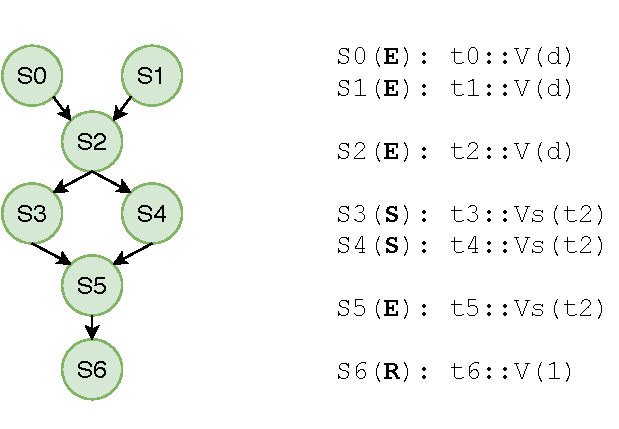
\includegraphics[width=.7\columnwidth]{./src/figure/graph-example.pdf}
\caption{A fusible section for the HorseIR program in \refFig{fig:motivation_horseir}. The
text format on the right hand side is \texttt{<statement>(<group>): <variable>::<shape>}.}
\label{fig:fusion_example}
\end{figure}

Given the HorseIR program in \refFig{fig:motivation_horseir}, our algorithm identifies a
fusible section shown in \refFig{fig:fusion_example}. Initially, the variable \texttt{c0}
is assigned a dynamic vector shape with unique ID, \texttt{V(d)}, as the exact size depends
on the input table. Next, the 3 element-wise functions in statements \texttt{S0},
\texttt{S1}, and \texttt{S2} propagate the vector shape \texttt{V(d)} according to the shape
rules. Both compressions in \texttt{S3} and \texttt{S4} generate a new shared scan shape
\texttt{Vs(t2)} as they both use the same boolean mask. The following binary function
uses this equality to correctly infer its output shape. Finally, the reduction function
\texttt{@sum} returns a vector with one element. Note that all functions in the computed
fusible section share the same loop range, \texttt{V(d)}.

The code in \refFig{fig:motivation_c} shows the generated C code for the complete
fusible section. Note the presence of an internal condition for the boolean selection
and the accumulator for the reduction. Details of the code generation strategy for fusible
sections are found in \refSec{Sec:codegen}.

% We mainly focus on how to identify fusible subgraphs and generate efficient code correctly.
%\todo{Add an example with a colored CFG tree to show which sections of the tree can be fused.}
% \subsection{Key Parts of the Analysis}

% \hanfeng{You may need to read its source code to see the complete algorithm.
% Sorry for the inconvenience.  It will be changed to a nice format with the latex
% algorithm package later.}



%%% Translated to an algorithm version
%% \begin{lstlisting}[mathescape=true, float=htbp, frame=single]
%% entry:
%%     id $\gets$ 1
%%     depth $\gets$ 0
%%     map $\gets$  $\varnothing$
%%     foreach node A in reversed topological order{
%%         if( !isVisited(A) ) {
%%             if ( A's op is a Reduction ){
%%                 section $\gets$ findFromReduction(A)
%%             }
%%             else {
%%                 section $\gets$ findFusibleSection(A,id)
%%             }
%%             if section is not an empty list
%%                 id $\gets$ id + 1
%%         }
%%     }
%% 
%%     function findFusibleSection(A, id){
%%         setVisited(A)
%%         isFusible = isOpInGroupWithoutR(A)
%%         if(isFusible){
%%             foreach node B in defStmts(A){
%%                 if( B has one use )
%%                     return  {A} $\cup$ findFusibleSection(A, id)
%%                 else{
%%                     if( B is not in map ){
%%                         list $\gets$ findFusibleSection(B, id)
%%                         insert the pair (B, list) into the map
%%                     }
%%                     else list $\gets$ map.get(B)
%%                     return {A} $\cup$ list
%%                 }
%%             }
%%         }
%%         return an empty set
%%     }
%% 
%%     function findFromReduction(A,id){
%%         setVisited(A)
%%         if (size of defStmts(A) is 1){
%%             return {A} $\cup$ findFusibleSection(getDefStmt(A,id))
%%         }
%%         else return {A}
%%     }
%% \end{lstlisting}



%\subsection{Conformable Operations in Groups} \label{SubSec:groups}

% Before generating C code correctly, we need shape rules defined in
% \refTab{table:example_elementwise} for elementwise functions.
% All cases can be determined statically except when both sides are vectors and a
% check for the both sizes is required.

% A set of well-defined primitive functions can be classified into groups
% because of their similar behaviours.  In HorseIR, a function has a fixed
% number of arguments, however, it is allowed to process arguments with
% different shapes.  For instance, \refTable{example:mul} shows the shape rules
% of the multiplication function, \texttt{mul}, having the two arguments which
% can be either a scalar or a vector.

% TODO: show the number of functions in groups 

% \todo{Replace the whole section by using more precise shape abstractions defined before.}

% \todo{Add description for vectors and lists.}

% It should be noted that the loop size is equal to the length of the boolean
% vector so that the condition vector can fit the entire loop correctly.  If two
% shapes with different condition aliases, they have to be conservatively
% considered as different shapes so that a failed shape is returned.
% Therefore, there are several kinds of results after the shape rules:

% \begin{itemize}
% \item \textbf{normal shape} for constant, symbolic, and selection sizes;
% \item \textbf{not conformable but continue} (NCC) for the failure of the shape propagation, but a new symbolic shape is assigned;
% \item \textbf{not conformable and abort} (NCA) for the failure of the shape propagation and the analysis aborts;
% \end{itemize}

% TODO: Type rules for each functions

% \todo{Algorithms for shape propagation.}


\section{Code Generation Strategies} \label{Sec:codegen}
Our code generation strategy follows a pattern based approach for fused sections,
whereas normal (non-fused) code calls optimized library functions. First, each fused section
is associated with a fusion node, the nodes are optimized, and lastly the code
is emitted.

%%% In this section we first introduce fusion node which collects the meta
%%% information of a fusible section.  Then, we present our implementation
%%% for constructing fusion nodes.  Finally, we generate code from fusion nodes.

\subsection{Fusion Nodes}

Each fused section is associated with a fusion node, a collection of metadata used
for generating the loop. For each section, we traverse the statements and collect:
(1) loop bounds; (2) fused expressions; (3) boolean mask (if any); and (4) reduction
operation (if any). The set of properties determines which code generation pattern
is used.

%% In this section we introduce fusion node for collecting the meta information of
%% a fusible section, and the code generation from fusion nodes.

%% One fusible section has one fusion node.
%% A fusion node needs to record the basic meta information which can be used to
%% construct a valid loop.  Thus, it has to traverse from the start statement of
%% the fusible section up to its predecessors until the last statement in the
%% fusible section.

%% During the traverse, the node keeps the loop head information including the size of
%% the loop, the condition mask if applicable, and whether it is a section for lists.
%% Meanwhile, it has to scan statement expressions to generate corresponding
%% expressions for both left-hand and right-hand side expressions by given type
%% and shape information.
%%% Q: Do we need to explain more?

%% \begin{figure}[htbp]
%% \begin{verbatim}
%%     {
%%       "loop_head": {
%%         "loop_size"   : string,
%%         "loop_cond"   : string,
%%         "loop_isList" : boolean
%%       },
%%       "loop_body": {
%%         "expr_lhs" : string,
%%         "expr_rhs" : string,
%%         "expr_tmp" : string[]
%%       },
%%       "start_stmt": stmt
%%     }
%% \end{verbatim}
%% \caption{Components of a simple loop for fusion.}
%% \label{fig:fusion_node_json}
%% \end{figure}

%%% A fusion node consists of a set of the following fields to save the meta
%%% information for a fusible section.

%%% \begin{description}
%%% \item[\texttt{loop_head}] describes the head of loop iteration including loop
%%% size, condition, and check for lists.
%%% 
%%% \begin{itemize}
%%% \item $loop\_size$: the number of loop iterations
%%% \item $loop\_cond$: an if-condition inside the loop
%%% \item $loop\_isList$: whether the loop is for list or vector
%%% \end{itemize}
%%% 
%%% \item[\texttt{loop_body}] represents the main computation of the loop which
%%% contains the following components.
%%% 
%%% \begin{itemize}
%%% \item $expr\_lhs$: left hand side expression 
%%% \item $expr\_rhs$: right hand side expression
%%% \item $expr\_tmp$: a list of temporary results
%%% \item $is\_r$: whether the start statement has a reduction operation
%%% \end{itemize}
%%% 
%%% \end{description}

%%% Note that the value of $loop\_cond$ is allowed to be empty that means there is
%%% no loop condition involved.
%%% 
%%% \subsection{Node Information Retrieval}
%%% 
%%% With a given fusion section, we fetch the information of its fusion node as described in
%%% \refAlgo{fetch_info}.
%%% 
%%% \todo{The algorithm has been commented out because it is hard to make it a
%%% short algorithm (too verbose). Will discuss with Alex to make this part clear.}

%%% \begin{lstlisting}
%%% entry:
%%%     Input: Given a fusion section (section) with a start statement (start)
%%%     Output: A fusion node
%%%     initialize a fusion node n
%%%     if (start is raze)
%%%         genNodeList(start, section)
%%%     else
%%%         genNodeVector(start, section)
%%% 
%%%     genNodeVector(stmt, section){
%%%         n.loop_size = genSize(stmt)
%%%         n.loop_isList = false
%%%         if(hasScanShape(stmt))
%%%             n.loop_cond = genNodeVector(getScanAlias(stmt),section)
%%%         else
%%%             n.loop_cond = ""
%%%         if(isReduction(stmt)) {
%%%             n.is_r = true
%%%             n.expr_lhs = genRop(stmt)
%%%             setVisited(stmt)
%%%             genNodeVectorRHS(getDefStmts(stmt)[0])
%%%         }
%%%         else {
%%%             n.is_r = false
%%%             n.expr_lhs = genTargetWithIndex(stmt)
%%%             n.expr_rhs = genNodeVectorRHS(stmt)
%%%         }
%%%     }
%%% 
%%%     genNodeVectorRHS(stmt, section){
%%%         setVisited(stmt)
%%%         def = getDefStmt(stmt)
%%%         if (def \in section){
%%%             if (map contains the def)
%%%                 return getOpMacro(stmt)+"("+map.get(def)+")"
%%%             if(hasOneChild(def))
%%%                 return getOpMacro(stmt)+"("+genNodeVectorRHS(def, section)+")"
%%%             else {
%%%                 tid = genTempId()    // a unique id
%%%                 tmp = tid + "=" + genNodeVectorRHS(def)
%%%                 map.insert(def, tid)
%%%                 expr_tmp.add(tmp)
%%%             }
%%%         }
%%%         else
%%%             return getOpMacro(stmt)+"("+genVectorExpr(stmt)+")"
%%%     }
%%% 
%%%     genNodeList(start, section){
%%%     }
%%% 
%%% \end{lstlisting}
 

%%% \begin{description}
%%% \item[Step 0:]
%%%     Determine if it is a fusion section for list, if true, goto Step X
%%% \item[Step 1:]
%%%     Identify the target (i.e. \texttt{expr_lhs}) which is stored in the start statement:
%%%     if a reduction operation is found, a scalar return is generated.
%%% \item[Step 2:]
%%% \end{description}

%%% \headstep{Collecting loop head.}

%%% \headstep{Collecting loop expression.}

\subsection{Code Generation for Vectors} \label{SubSec:CodeGen}

%% \begin{verbatim}
%% -------------------------------------------
%% Start stmt | Has Scan? | C Code
%% -------------------------------------------
%%    R       |  yes      |  ...
%%            |  no       |  ...
%% -------------------------------------------
%%    No R    |  yes      |  ...
%%            |  no       |  ...
%% -------------------------------------------
%% \end{verbatim}

\begin{figure}[htbp]
\par\noindent\rule{\columnwidth}{0.6pt}
% first row
\begin{subfigure}[t]{.45\columnwidth}
\begin{small}
\begin{verbatim}
// reduction: YES
// scan: YES
for(i=0; i<len; i++){
  if(cond[i]){
      z = z Rop expr_rhs;
  }
}
z = Rfinal(z);
\end{verbatim}
\end{small}
\caption{Case 0} \label{fig:codegen_c0}
\end{subfigure}
\hspace{1mm}
\rulesep
\hspace{2mm}
\begin{subfigure}[t]{.45\columnwidth}
\begin{small}
\begin{verbatim}
// reduction: YES
// scan: NO
for(i=0; i<len; i++){

  z = z Rop expr_rhs;

}
z = Rfinal(z);
\end{verbatim}
\end{small}
\caption{Case 1} \label{fig:codegen_c1}
\end{subfigure}
\vspace{1mm}
\par\noindent\rule{\columnwidth}{0.6pt}
% second row
\begin{subfigure}[t]{.45\columnwidth}
\begin{small}
\begin{verbatim}
// reduction: NO
// scan: YES
c = 0;
for(i=0; i<len; i++){
  if(cond[i]){
    z[c++] = expr_rhs;
  }
}
\end{verbatim}
\end{small}
\caption{Case 2} \label{fig:codegen_c2}
\end{subfigure}
\hspace{1mm}
\rulesep
\hspace{2mm}
\begin{subfigure}[t]{.45\columnwidth}
\begin{small}
\begin{verbatim}
// reduction: NO
// scan: NO

for(i=0; i<len; i++){

  z[i] = expr_rhs;

}
\end{verbatim}
\end{small}
\caption{Case 3} \label{fig:codegen_c3}
\end{subfigure}
\vspace{1mm}
\par\noindent\rule{\columnwidth}{0.6pt}
\caption{Code generation for vectors. \texttt{Rop}: reduction operation; \texttt{Rfinal}: final reduction step (e.g. divide by element count); \texttt{z}: accumulator/output vector.} \label{fig:codegen_vectors}
\end{figure}

Code generation for fused vector operations follows 4 patterns depending on the presence
of reduction and boolean selection. Each iterates over the length of the list, fuses the
RHS expressions, and produces the appropriate output. Reduction nodes accumulate a scalar
value, while non-reduction nodes create a new vector. \texttt{Rfinal} performs the final
step of the reduction (e.g. dividing by the number of elements to compute an average).
In the case of compression, the condition is first evaluated and the RHS computed if
necessary. \refFig{fig:codegen_vectors} shows the variations of the code generation patterns.

Note that when generating parallel code for \refFig{fig:codegen_c2}, we employ a
strategy that:
(1) counts the number of true elements in each segment and computes an offset for
each segment; and
(2) divides the boolean vector into segments evenly based on the number of cores.
Each thread thus maintains a segment of the boolean vector independently. For all other
cases, typical parallel strategies are effective.

%%% \begin{algorithm}
%%% \SetAlgoLined
%%% \KwResult{Result}
%%% let op $\gets$ op\_name\;
%%% let x,y $\gets$ op\_args\;
%%% \Switch{op_kind}{
%%%   \Case{Unary Elementwise with E(op,x)}{
%%%     \Return{isScalar(x) ? op(x) : op($\vec{x}$)}\;
%%%   }
%%%   \Case{Binary Elementwise with E(op,x,y)}{
%%%     \eIf{isScalar(x)}{
%%%       \Return{isScalar(y) ? op(x,y) : op(x,$\vec{y}$)}\;
%%%     }{
%%%       \Return{isScalar(y) ? op($\vec{x}$,y) : op($\vec{x}$,$\vec{y}$)}\;
%%%     }
%%%   }
%%%   \Case{Reduction with R(op,x)}{
%%%     \Return{isScalar(x) ? op(=,x) : op(=,$\vec{x}$)}\;
%%%   }
%%%   \Case{Scan with S(m, x)}{
%%%     \Return{$\vec{x}$}\;
%%%   }
%%%   \Case{Indexing with $X$(x,y)}{
%%%     \Return{x($\vec{y}$)}\;
%%%   }
%%%   \Case{Special boolean with B(x,y) and op_name as func}{
%%%     \Return{isScalar(x) ? func(x,y) : func(x,$\vec{y}$)}\;
%%%   }
%%% }
%%% \caption{Code Generation for Sub-expressions.} \label{algo:expr}
%%% \end{algorithm}

\subsection{Generating Code for Lists}

%%% \begin{figure}[htbp]
%%% \par\noindent\rule{\columnwidth}{0.6pt}
%%% % first row
%%% \begin{subfigure}[t]{.45\columnwidth}
%%% \begin{verbatim}
%%% for(i=0;i<len;i++){
%%%   c = list[i]; // cell
%%%   // init t
%%%   for(j=0;j<c_len;j++){
%%%       t = t Rop(cell[j])
%%%   }
%%%   z[i] = Rfinal(t);
%%% }
%%% \end{verbatim}
%%% \caption{Code generation template.} \label{fig:codegen_list_temp}
%%% \end{subfigure}
%%% \hspace{1mm}
%%% \rulesep
%%% \hspace{2mm}
%%% \begin{subfigure}[t]{.45\columnwidth}
%%% \begin{verbatim}
%%% for(i=0;i<len;i++){
%%%   c = v[i]; // cell
%%%   t = 0;  // init for sum
%%%   for(j=0;j<c_len;j++){
%%%       t = t + age[c[i]];
%%%   }
%%%   avg[i] = t/c_len;
%%% }
%%% \end{verbatim}
%%% \caption{Example code for \refFig{fig:list_horseir}} \label{fig:codegen_list_example}
%%% \end{subfigure}
%%% \vspace{1mm}
%%% \par\noindent\rule{\columnwidth}{0.6pt}
%%% \caption{Code generation for lists.} \label{fig:codegen_lists}
%%% \end{figure}

\begin{figure}[htbp]
\par\noindent\rule{\columnwidth}{0.6pt}
%[xleftmargin=.2\columnwidth]
\begin{small}
\begin{verbatim} 
for(i=0; i<list.len; i++){ /* loop over cells */
  cell = list[i]; /* fetch one cell */
  /* init t */
  for(j=0; j<cell.len; j++){ /* loop over content */
      t = t Rop (cell[j])
  }
  z[i] = Rfinal(t); /* store final value */
}
\end{verbatim}
\end{small}
\vspace{-1mm}
\par\noindent\rule{\columnwidth}{0.6pt}
\caption{Code generation for lists. \texttt{Rop}: reduction operation; \texttt{Rfinal}: final reduction step (e.g. divide by element count); \texttt{t}: cell accumulator; \texttt{z}: output vector.} \label{fig:codegen_lists}
\end{figure}

List fusion nodes compute a single value per list cell and return a vector. \refFig{fig:codegen_lists} shows the code generation pattern for lists. As seen in
the figure, there are two loops present: an outer loop iterating over cells and an
inner loop computing the reduction expression for each cell.

% \refFig{fig:codegen_list_example} is an example code in C for
% \refFig{fig:list_horseir}.

Note that the ratio of \texttt{list.len} and \texttt{cell.len} may vary greatly.
When parallel code is generated, we may therefore parallelize the outer or inner loop
depending on the data. In our implementation, we use a simple runtime heuristic based
on the size ratio to choose which loop runs in parallel.

\subsection{Further Fusion Opportunities}

Fusible sections can be further fused if:
(1) they share the same loop head, and
(2) there is no data dependence between the loop bodies.
This is particularly useful and common in column-based IMDBs where data is fetched
from multiple independent columns using a single array of indices (e.g. the result
of a join). It also improves parallelization as the number of synchronization barriers
is reduced.

%  A tuple of a code generation rule is
%  
%  \begin{center}
%  T = \tupleSingle{$op\_kind$}{$op\_name$}{$n$}{$cond$}{$expr$\{, $expr$\}}\\
%  \end{center}
%  
%  where
%  
%  \begin{itemize}
%  \item $op\_kind$: the kind of the operation;
%  \item $op\_name$: the name of the operation;
%  \item $n$:  a loop from 0 (inclusive) to n (exclusive);
%  \item $cond$: an if-condition inside the loop; and
%  \item $expr$\{, $expr$\}: a list of expressions as input for the main computation in the loop body;
%  \end{itemize}
%  
%  In the first example as follows, $E_2$ means the binary elementwise operation;
%  the condition is set to null; and the main computation attributes to the
%  addition of x[i] and y[i].  On the right side, we can see that its
%  corresponding code generated from the given tuple, where the loop is generated
%  with a range of [0,n) and the result of the addition is saved to a target
%  array.
%  
%  \vv
%  
%  % textwidth: two columns
%  
%  \noindent
%  \begin{minipage}{.53\columnwidth}
%  \begin{tabular}{l}
%  \textbf{Example 1:} \\
%  \tuple{$E_2$}{PLUS}{n}{null}{x[i]}{y[i]}
%  \end{tabular}
%  \end{minipage}
%  %\hfill
%  \begin{minipage}{.37\columnwidth}
%  \begin{tabular}{|c}
%  %\hspace{1mm}
%  \begin{minipage}{\columnwidth}
%  \begin{verbatim}
%  for(int i=0; i<n; i++){
%    targ[i] = x[i] + y[i];
%  }
%  \end{verbatim}
%  \end{minipage}
%  \end{tabular}
%  \end{minipage}
%  
%  \vspace{4mm}
%  
%  In the second example below, $R$ means the reduction; a condition is associated
%  with a variable $b$; and the expression is  a multiplication of \texttt{x[i]}
%  and \texttt{y[i]}. On the right side, we can see that the loop body contains a
%  boolean mask \texttt{b[i]} with the main computation expression inside the true
%  block.
%  
%  \vv
%  
%  \noindent
%  \begin{minipage}{.53\columnwidth}
%  \begin{tabular}{l}
%  \textbf{Example 2:} \\
%  \tupleSingle{R}{SUM}{$n$}{$b$}{mul(x[i],y[i])}
%  \end{tabular}
%  \end{minipage}
%  %\hfill
%  \begin{minipage}{.37\columnwidth}
%  \begin{tabular}{|c}
%  %\hspace{1mm}
%  \begin{minipage}{\columnwidth}
%  \begin{verbatim}
%  for(int i=0; i<n; i++){
%    if(b[i]){
%      targ += x[i] * y[i];
%    }
%  }
%  \end{verbatim}
%  \end{minipage}
%  \end{tabular}
%  \end{minipage}
%  
%  \vv
%  
%  \refTab{Tab:op_list} shows the information of classified primitive functions.  The number of operands varies so that the number of elements in a tuple can be different.
%  
%  \noindent
%  \begin{table}[htbp]
%  \centering
%  \caption{List of kinds of primitive functions} \label{Tab:op_list}
%  \begin{tabular}{|c|c|c|}
%  \hline
%  Kind     & Name               & \# of Operands \\ \hline
%  $E_1$    & Unary elementwise  & 1 \\ \hline
%  $E_2$    & Binary elementwise & 2 \\ \hline
%  $R$      & Reduction          & 1 \\ \hline
%  $C$      & Compression        & 2 \\ \hline
%  \end{tabular}
%  \end{table}
%  
%  \subsection{Elementwise Function - Dyadic}
%  
%  \refTab{Tab:gen_elem_dyadic} presents the shape rules of dynamic elementwise functions after the conformability analysis.  Let \TupleETwo{0} denote the first rule inside the table, then we can have all 9 cases with their corresponding code generation tuples in \refTab{Tab:gen_rules_elem_dyadic}.
%  
%  \begin{table}[htbp]
%  \centering
%  \caption{Elementwise Functions - Dyadic} \label{Tab:gen_elem_dyadic}
%  \vv
%  \begin{tabular}{c||c|c|c}
%  \hline
%  x op y & \scan{$b_0$}{$n_0$} & $m_0$ ($m_0 \neq 1$) & 1 \\
%  \hline \hline
%  \scan{$b_1$}{$n_1$} & \scan{$b_0$}{$n_0$} & Fail & \scan{$b_1$}{$n_1$} \\
%  \hline
%  $m_1$ ($m_1 \neq 1$) & Fail & $m_0$ & $m_1$ \\
%  \hline
%  1     & \scan{$b_0$}{$n_0$} & $m_0$ & 1 \\
%  \hline
%  \end{tabular}
%  \end{table}
%  
%  
%  \begin{table}[htbp]
%  \centering
%  \caption{Code Generation Rules for Dyadic Elementwise Functions } \label{Tab:gen_rules_elem_dyadic}
%  \vv
%  \begin{tabular}{c||c|c|c}
%  \hline
%  x op y & \scan{$b_0$}{$n_0$} & $m_0$ ($m_0 \neq 1$) & 1 \\
%  \hline \hline
%  \scan{$b_1$}{$n_1$} & \TupleETwo{0} & \TupleETwo{1} & \TupleETwo{2} \\
%  \hline
%  $m_1$ ($m_1 \neq 1$) & \TupleETwo{3} & \TupleETwo{4} & \TupleETwo{5} \\
%  \hline
%  1     & \TupleETwo{6} & \TupleETwo{7} & \TupleETwo{8} \\
%  \hline
%  \end{tabular}
%  \\ \vv
%  \begin{tabular}{|c|l|l|}
%  \hline
%  Case ID & \multicolumn{1}{c|}{Code Generation Tuple} & \multicolumn{1}{c|}{Output Expr} \\
%  \hline
%  \TupleETwo{0} & \tuple{$E_2$}{$op$}{$n_0$}{$b_0$}{$x[i]$}{$y[i]$} & $x[i]\ op\ y[i]$  \\ \hline
%  \TupleETwo{1} & ------ & ------ \\ \hline
%  \TupleETwo{2} & \tuple{$E_2$}{$op$}{$n_0$}{$b_0$}{$x$}{$y[i]$}    & $x\ op\ y[i]$     \\ \hline
%  \TupleETwo{3} & ------ & ------ \\ \hline
%  \TupleETwo{4} & \tuple{$E_2$}{$op$}{$n_0$}{$null$}{$x[i]$}{$y[i]$}& $x[i]\ op\ y[i]$  \\ \hline
%  \TupleETwo{5} & \tuple{$E_2$}{$op$}{$n_0$}{$null$}{$x$}{$y[i]$}   & $x\ op\ y[i]$  \\ \hline
%  \TupleETwo{6} & \tuple{$E_2$}{$op$}{$n_0$}{$b_0$}{$x[i]$}{$y$}    & $x[i]\ op\ y$  \\ \hline
%  \TupleETwo{7} & \tuple{$E_2$}{$op$}{$n_0$}{$null$}{$x[i]$}{$y$}   & $x[i]\ op\ y$  \\ \hline
%  \TupleETwo{8} & \tuple{$E_2$}{$op$}{$null$}{$null$}{$x[i]$}{$y$}  & $x[i]\ op\ y$  \\ \hline
%  \end{tabular}
%  \end{table}
%  
%  
%  %Row 1
%  %
%  %\begin{itemize}
%  %\item \TupleCase{\scan{$b_1$}{$n_1$}}{\scan{$b_0$}{$n_0$}} = \tuple{$E_2$}{$op$}{$n_0$}{$b_0$}{$x[i]$}{$y[i]$}
%  %\item \TupleCase{\scan{$b_1$}{$n_1$}}{$m_0$} = N/A
%  %\item \TupleCase{\scan{$b_1$}{$n_1$}}{1} = \tuple{$E_2$}{$op$}{$n_0$}{$b_0$}{$x$}{$y[i]$}
%  %\end{itemize}
%  %
%  %Row 2
%  %
%  %\begin{itemize}
%  %\item \TupleCase{$m_1$}{\scan{$b_0$}{$n_0$}} = N/A
%  %\item \TupleCase{$m_1$}{$m_0$} = \tuple{$E_2$}{$op$}{$n_0$}{$null$}{$x[i]$}{$y[i]$}
%  %\item \TupleCase{$m_1$}{1} = \tuple{$E_2$}{$op$}{$n_0$}{$null$}{$x$}{$y[i]$}
%  %\end{itemize}
%  %
%  %Row 3
%  %
%  %\begin{itemize}
%  %\item \TupleCase{1}{\scan{$b_0$}{$n_0$}} = \tuple{$E_2$}{$op$}{$n_0$}{$b_0$}{$x[i]$}{$y$}
%  %\item \TupleCase{1}{$m_0$} = \tuple{$E_2$}{$op$}{$n_0$}{$null$}{$x[i]$}{$y$}
%  %\item \TupleCase{1}{1} = \tuple{$E_2$}{$op$}{$null$}{$null$}{$x[i]$}{$y$}
%  %\end{itemize}
%  
%  \subsection{Elementwise Function - Monadic}
%  
%  \refTab{Tab:gen_elem_monadic} presents the shape rules of monadic elementwise functions after the conformability analysis.  Let \TupleEOne{0} denote the first rule inside the table, then we can have all 3 cases with their corresponding code generation tuples in \refTab{Tab:gen_rules_elem_monadic}.
%  
%  \begin{table}[ht!]
%  \centering
%  \caption{Elementwise Functions - Monadic} \label{Tab:gen_elem_monadic}
%  \vv
%  \begin{tabular}{c|c|c|c}
%  \hline
%  op x & \scan{$b_0$}{$n_0$} & $m_0$ ($m_0 \neq 1$) & 1 \\
%  \hline
%         & \scan{$b_0$}{$n_0$} & $m_0$ & 1 \\
%  \hline
%  \end{tabular}
%  \end{table}
%  
%  \begin{table}[ht!]
%  \centering
%  \caption{Code Generation Rules for  Monadic Elementwise Functions} \label{Tab:gen_rules_elem_monadic}
%  \vv
%  \begin{tabular}{c|c|c|c}
%  \hline
%  op x & \scan{$b_0$}{$n_0$} & $m_0$ ($m_0 \neq 1$) & 1 \\
%  \hline
%         & \TupleEOne{0} & \TupleEOne{1} & \TupleEOne{2} \\
%  \hline
%  \end{tabular}
%  \\ \vv
%  \begin{tabular}{|c|l|}
%  \hline
%  Case ID & \multicolumn{1}{c|}{Code Generation Tuple} \\
%  \hline
%  \TupleEOne{0} & \tupleSingle{$E_1$}{$op$}{$n_0$}{$b_0$}{$x[i]$}  \\ \hline
%  \TupleEOne{1} & \tupleSingle{$E_1$}{$op$}{$n_0$}{$null$}{$x[i]$} \\ \hline
%  \TupleEOne{2} & \tupleSingle{$E_1$}{$op$}{$null$}{$null$}{$x$}     \\ \hline
%  \end{tabular}
%  \end{table}
%  
%  \subsection{Reduction}
%  
%  An operation reduction can be performed the code below which sums up total value in an integer vector \texttt{x}.
%  
%  
%  \begin{minipage}{.4\columnwidth}
%  \begin{verbatim}
%  S1: sum = 0;
%  S2: for(int i=0; i<n; i++){
%  S3:     sum = sum + x[i];
%  S4: }
%  \end{verbatim}
%  \end{minipage}
%  \hfill
%  % https://tex.stackexchange.com/a/29237
%  \begin{minipage}{.4\columnwidth}
%  \small
%  \begin{tikzpicture}
%  \node[draw, align=left] at (0,0) {\baselineskip=20pt L0: sum_0 = 0;\\ L1: sum_1 = sum_0 + x[0]; \\ L2: sum_2 = sum_1 + x[1]; \\ L3: sum_3 = sum_2 + x[2]; \\ ...};
%  \draw [->, densely dotted, blue, line width=1pt] (-0.8,0.6)   -- (0.1,0.45);
%  \draw [->, densely dotted, blue, line width=1pt] (-0.8,0.25)  -- (0.1,0.1);
%  \draw [->, densely dotted, blue, line width=1pt] (-0.8,-0.15) -- (0.1,-0.3);
%  \draw [->, densely dotted, blue, line width=1pt] (-0.8,-0.5)  -- (0.1,-0.65);
%  \end{tikzpicture}
%  \end{minipage}
%  \begin{minipage}{.4\columnwidth}
%  \end{minipage}
%  
%  \vv
%  
%  The variable \texttt{sum} in the statement \texttt{S3} has the data dependency
%  on the previous value of \texttt{sum}.  Therefore, fusing primitive functions
%  after the reduction is unfeasible.
%  
%  
%  \begin{table}[ht!]
%  \centering
%  \caption{Reduction} \label{Tab:gen_reduction}
%  \vv
%  \begin{tabular}{c|c|c|c}
%  \hline
%  op x & \scan{$b_0$}{$n_0$} & $m_0$ ($m_0 \neq 1$) & 1 \\
%  \hline
%         & 1 & 1 & 1 \\
%  \hline
%  \end{tabular}
%  \end{table}
%  
%  \begin{table}[ht!]
%  \centering
%  \caption{Code Generation Rules for Reduction} \label{Tab:gen_rules_reduction}
%  \vv
%  \begin{tabular}{c|c|c|c}
%  \hline
%  op x & \scan{$b_0$}{$n_0$} & $m_0$ ($m_0 \neq 1$) & 1 \\
%  \hline
%         & \TupleEOne{0} & \TupleEOne{1} & \TupleEOne{2} \\
%  \hline
%  \end{tabular}
%  \\ \vv
%  \begin{tabular}{|c|l|}
%  \hline
%  Case ID & \multicolumn{1}{c|}{Code Generation Tuple} \\
%  \hline
%  \TupleEOne{0} & \tupleSingle{$R$}{$op$}{$n_0$}{$b_0$}{$x[i]$}  \\ \hline
%  \TupleEOne{1} & \tupleSingle{$R$}{$op$}{$n_0$}{$null$}{$x[i]$} \\ \hline
%  \TupleEOne{2} & \tupleSingle{$R$}{$op$}{$null$}{$null$}{$x$}     \\ \hline
%  \end{tabular}
%  \end{table}




\section{Evaluation} \label{Sec:evaluation}
In this section we evaluate the performance of our optimizations by conducting
experiments on the TPC-H benchmark. 

\subsection{Methodology}

\head{Experimental setup.}
We run all benchmarks under Ubuntu 16.04.6 LTS on a server which has 4 Intel
Xeon E7-4850 2.00GHz (total 40 cores with 80 threads) and 128 GB RAM.
We use GCC compiler with the version \textit{v8.1.0} to compile the generated C
code after optimizations with a maximum optimization option \texttt{-O3} and
enabled \texttt{-march=native}.
We use the latest MonetDB \cite{IdreosS2012} released as \textit{Apr2019} with
version v11.33.3, as a baseline to compare with the following HorseIR versions:
(1) HorseIR-noopt: a naive version without any optimizations;
(2) HorseIR-opt1 : an optimized version with element-wise and pattern-based
fusion enabled as presented in the previous work~\OldPaper; and
(3) HorseIR-opt2 : optimization uses the approach presented in this paper.

\head{Execution time.}
Our results present the core execution time of the database query. That is, compilation time, the time to load the input data into memory and the time to output results are not considered, as we want to zoom on the effects of the optimization.  
The results present the average over 15 executions for each query.

% \head{Micro-benchmarks.}

\head{TPC-H SQL benchmarks.}
TPC-H \cite{TPCH2017} is a widely used SQL benchmark suite for analytical data
processing simulating real Business to Consumer (B2C)
database applications. The database has 8 tables over which 22 queries are
defined.  The database size can be varied by indicating a  \textit{scale factor} (SF).
For example, a scale factor of 1 (i.e. SF1) means 1GB of input
data. With an increasing scale factor, (nearly) each of the tables holds more
data records. Our results are for SF1 but initial results on larger scale
factors show similar results.

For this paper, we have selected 8 of the 22 queries (q1/4/6/12/14/16/19/22). These are the queries where the basic built-in functions that we aim to fuse have a major impact on the query execution time. In particular, these queries have a maximum of 2 joins. Joins are very expensive, and in queries with more than 2 joins, the join execution takes up most of the time, thus, the optimizations presented in \OldPaper and in this paper have less impact.   Future work will look more closely at fusion potential for join operations.  

%% In our experiments, we use a number of SFs growing exponentially, i.e.
%% SF1/2/4/8/16, to test the scalability of the generated parallel code.

% \subsection{Micro-benchmarks Results}

\subsection{Execution Time Results}

\begin{figure*}[htbp]
\centering
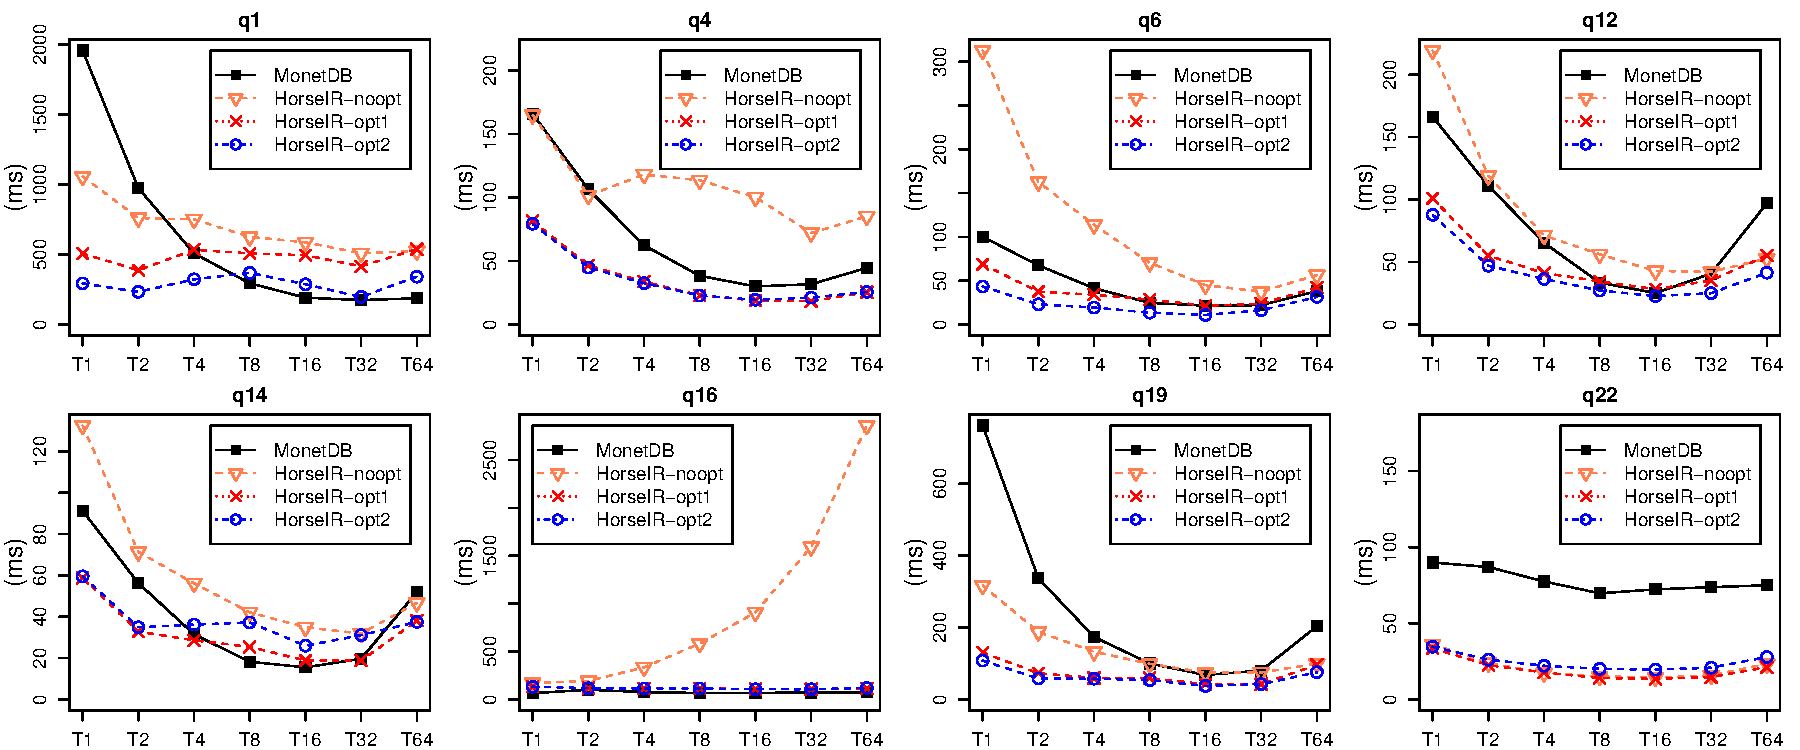
\includegraphics[width=\textwidth]{./src/figure/sf1-v2.pdf}
\caption{The result of TPC-H queries with 1GB input data (SF1).}
\label{fig:tpch_result}
\end{figure*}


\refFig{fig:tpch_result} shows the execution times using MonetDB, HorseIR-noopt,
HorseIR-opt1, and HorseIR-opt2 on SF1 with increasing number of threads. 
Execution time generally decreases with increasing number of threads up to a
thread threshold except for q16. The sweet spot for both MonetDB and HorseIR
where the best performance is achieved, is at around 16 threads. Thus, using
parallel execution is beneficial for most of the queries. The problem with q16
is that it has many cells (18314) with only a very small vector in each cell
(average size 6.5). Thus, q16 cannot take advantage of parallelization as it
focuses on the vectors in the cells. 

HorseIR-noopt has the worst performance in most cases showing that optimization
techniques are crucial when trying to exploit array-based languages for query
execution. The two HorseIR-opt versions are generally not as sensitive to the
number of threads as MonetDB, which shows quite bad performance for many
queries when there are only a few threads. 
When looking only at the optimal thread level around 16, MonetDB shows the best
performance for one query, HorseIR-opt1 for one query, HorseIR-opt2 for two
queries, HorseIR-opt1 and HorseIR-opt2 for two queries, and all three behave
very similarly for two queries. That is, there are only 2 queries where our
approach is worse than one of the other approaches, and that only by a small
margin.

\begin{figure}[htbp]
\centering
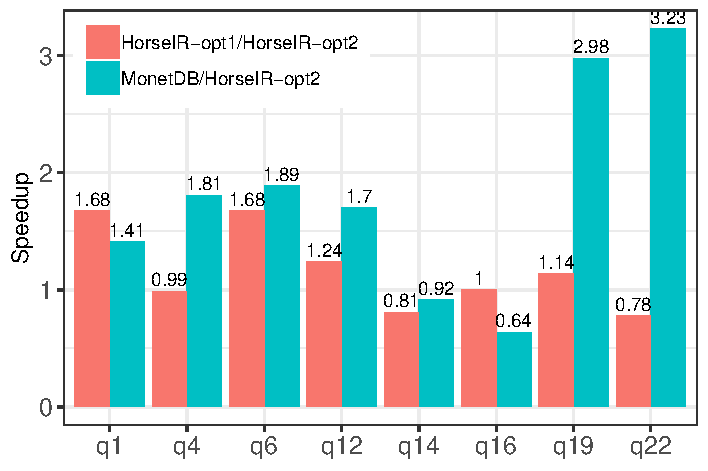
\includegraphics[width=.9\columnwidth]{./src/figure/sf1-speedup.pdf}
\caption{Geometric means of TPC-H queries with 1GB input data (SF1).}
\label{fig:tpch_sf1_speedup}
\end{figure}

In order to better understand the performance benefit of our approach across all thread levels, 
\refFig{fig:tpch_sf1_speedup}  presents  the geometric mean for the comparison
between HorseIR-opt2 in regard to HorseIR-opt1 and MonetDB. 
HorseIR-opt2 provides an improvement over MonetDB (mean > 1) for all but one
query and the improvement is quite significant. 

Comparing with HorseIR-opt1, we improve for four queries, are the same for two
queries, and are worse for two queries. The average execution times of
HorseIR-opt2 are about 12\% faster than HorseIR-opt1 in terms of geometric
means.

\textit{When we are better.}
For q1, our optimizer is able to identify eight fusible sections that are
further merged into a big loop that helps improve the overall performance.
For q6, two blocks of element-wise functions that are separated by
non-element-wise statement (i.e., \texttt{@compress}) are fused together. In
both cases, intermediate results are avoided and performance improved.
For q12 and q19, more statements are fused and less intermediate results
created but the effect is weaker.

\textit{When we are worse.}
For q14 and q22, the loop sizes of fused statements are relatively small with
long expressions in the loop body. Thus, fusion makes things more complicated
without the benefit of iterating less times. 

\textit{When we behave similarly.}
For queries q4 and q16, the filters are very selective and only a few rows
qualify. Thus, fusing loops has little benefit but also does not harm the
execution.

%%% The main computation part of the queries have operators unable to be fused.
%%% That means we can either improve the operators with efficient implementations
%%% or come up with a new group and a new analysis in order to achieve code fusion.



%%% \todo{The results of q1 and q14 are much slower than MonetDB, however, they are
%%% faster than MonetDB on the previous paper.  (Already send email to Andrew to ask
%%% for his help, maybe a RAM failure again)}

%%% \todo{Add scalability}

\subsection{Fusing Statements}

\begin{figure}[htbp]
\centering
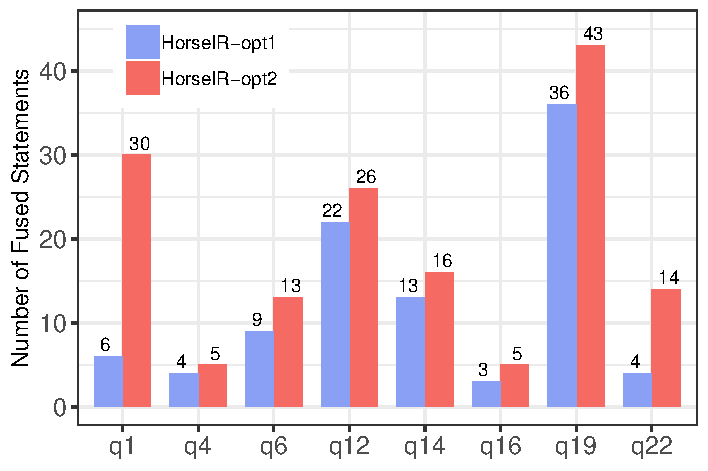
\includegraphics[width=.9\columnwidth]{./src/figure/bar-number.pdf}
\caption{Number of element-wise fused statements in HorseIR-opt1 and our new fusion in HorseIR-opt2.}
\label{fig:opt_number}
\end{figure}

\refFig{fig:opt_number} shows the the number of fused statements using
element-wise fusion in HorseIR-opt1 and the more general function fusion in
HorseIR-opt2.  Note that we do not show pattern-based fusion because both
HorseIR-opt1 and HorseIR-opt2 use the same patterns. 

We can see that our approach always fuses more statements than HorseIR-opt1.
For q1 and q22, there exist a large set of list-related statements that can be
fused together without the need of using patterns.  Furthermore, our optimizer
performs a fair amount of fusions with mixed function types, such as
element-wise and reduction functions. 

However, as we have seen in the previous analysis, fusing is not always
beneficial. For instance, in q22, we perform many more fusions than
HorseIR-opt1, but the loops have now complex expressions which actually results
in worse performance compared to the HorseIR-opt1. 



%%% In the query q1, the number of patterns are significantly reduced because a set
%%% of fusion nodes can be further merged into a single loop due to the same loop
%%% structure.  In q6, the pattern for common masks are removed because the result
%%% of boolean selection will be reduced into a single number so that their the
%%% intermediate results should be discard.


%%% \begin{table}[htbp]
%%% \centering
%%% \caption{Number of statements fused in benchmark queries under two versions of optimizations}
%%% \label{table:opt_number}
%%% \begin{tabular}{|c||c|c|c|c|}
%%% \hline
%%% & \multicolumn{2}{c||}{HorseIR-opt1} & \multicolumn{2}{c|}{HorseIR-opt2} \\ \hline
%%% Query & Patterns & Elementwise & Patterns & Fusion \\ \hline
%%% \hline
%%% q1  & 11 & 2 & 3 & 1 \\ \hline
%%% q4  & 3 & 1 & 2 & 2 \\ \hline
%%% q6  & 1 & 1 & 0 & 1 \\ \hline
%%% q12 & 3 & 5 & 3 & 3 \\ \hline
%%% q14 & 2 & 4 & 2 & 4 \\ \hline
%%% q16 & 5 & 1 & 5 & 2 \\ \hline
%%% q19 & 2 & 6 & 1 & 6 \\ \hline
%%% q22 & 4 & 2 & 2 & 3 \\ \hline
%%% \end{tabular}
%%% \end{table}


\subsection{Discussion}

In summary, we can see that fusion across statements is beneficial in many
cases. However, we can see two situations, where one has to be more careful about
applying fusion. The first is that fusing too many statements might become
sub-optimal. We believe this is due to the increased pressure on register
allocation. Maybe one could create heuristics to determine a maximum number of
statements to be fused. 

The second situation arises when filtering conditions have a high selectivity,
e.g., when only 10 out of a million records qualify. Then the benefit of
avoiding intermediate results is negligible, while the overhead of code fusion
might become a factor. 
If one had enough information about the properties of the actual data, such
unnecessary fusions could be avoided. Therefore, introducing runtime
optimizations in order to decide when to use the optimized code is an
interesting avenue for future research. 






\section{Related Work} \label{Sec:relatedwork}
% \subsection{Fusion Teachniques}
% \subsection{Related Database Systems}

% \begin{description}
% \item[Lift with patterns] High-level synthesis of functional patterns with
%     Lift~\cite{Kristien19:LiftPatterns}.
% \item[WeldIR] Evaluating End-to-End Optimization for Data Analytics
%     Applications in Weld~\cite{Palkar18:Weld}.
% \item[Peloton] Our code generation fits the SIMD predicate evaluation used in
%     Peloton. That implies our code generation can be further improved with
%     lower but efficient instructions.
% \end{description}

% \todo{Add "How to Architect a Query Compiler, Revisited"~\cite{TahboubER18:Revisited}}
% \todo{Add "Generating code for holistic query evaluation"~\cite{}}

Fusion techniques are popular due to their success in reducing intermediate
results. This is especially true for compiled environments which easily
allow code fusion.

\head{Fusion in programming languages}

% Operator fusion is an effective technique for high-level programming languages,
% especially for array-based programming languages.

In the MATLAB-to-FORTRAN compiler~\cite{rose1999:techniques}, shape and size
information can be obtained from a conformability analysis with a set of
well-defined conformable operators for scalar, vector, and matrix.
However, no further operator fusions after conformability analysis are provided.

In the R programming language, a vectorizer is proposed for the built-in
function \texttt{Apply}~\cite{Wang2015:vectorization}. The function
\texttt{Apply} is similar to our list-based functions, which take
a function and a list of data inputs as parameters and repeatedly apply
the function. Their vectorizer involves both code and data transformation
while we focus on code optimization. Additionally, we explore a wider set
of built-in functions rather than only a single list-based function.

Ju et al.~\cite{ju1994:array} investigate built-in function fusion in a pure
array-based programming language, APL. They classify operators into categories
based on the features of the functions and present a model to help generate
parallel code when fusing built-in functions. Ching et al.~\cite{ChingZ12parallel}
use simple techniques to fuse arithmetic functions when compiling APL to parallel
C code. In contrast, our work is aimed at array-based programs generated from
SQL queries, considering functions important to database operators.

Similar to optimizations for arrays~\cite{KumarH14,FoleyH16matjuice},
we exploit type and shape information of arrays to generate efficient code.
But due to the high-level semantics of HorseIR programs, we avoid
complicated vectorization techniques~\cite{menon1999case,ChenKLH16}.

\head{Fusion in database query optimizations}

%As the previal of query compilers in database systems, it is important to
%exploit fusion opportunities in standard SQL queries in order to generate
%efficient code.

% fusing multiple relational operations.
%HIQUE~\cite{Krikellas10:HIQUE} generates C++ code using code templates for each operator.
% As can be seen, they share our goal of fusing operators. However, we approach
% the problem from a static analysis perspective that operates on the IR-level
% rather than directly on the execution plan.

\new{
When loop fusion is applied to query related code, it is complicated to
identify optimization opportunities by using a predefined set of rules.
The DBLAB/LB query compiler~\cite{ShaikhhaKPBD016} provides fusion rules for
different loop fusion algorithms to generate optimized code
\cite{Shaikhha2018:LoopFusion}.
WeldIR~\cite{Palkar18:Weld} adopts rule-based optimizations for element-wise
and common-loop-head fusion.
HorseQC\cite{FunkeBNMT18:HorseQC} and HIQUE~\cite{Krikellas10:HIQUE} present
rule-based fusion strategies.  
However, just as the patterns in \OldPaper, the rule-based approach is
challenging to generalize. % page 21
}

\new{
HyPer~\cite{Neumann2011:HyPer}, an in-memory database system, adopts a data-centric
model when compiling SQL queries to LLVM code. They developed a greedy
algorithm to produce/consume operators directly in an execution plan in order
to fuse relational operations directly.
Peloton~\cite{Menon2017:Peloton} considers operator fusion for operators within a pipeline.
The stream-fusion~\cite{Shaikhha2018:LoopFusion} needs to define extra
fusion-related constructs for producing, consuming, unfolding, and destroying a
collection.
We have a different fusion strategy by providing a systematic approach which
collects precise shape information on a well-defined array-based language for
automatic fusion.}

%%% The Peloton in-memory DBMS~\cite{Menon2017:Peloton} considers operator
%%% fusion for operators within a pipeline. Again, the use quite specialized fusion
%%% rules, while we provide a more general optimization approach.
%%% On the other hand, their core strategy, SIMD predicate evaluation, can
%%% be applied to our code generation directly.

\head{Performance-oriented Systems}

%%% Weld~\cite{Palkar18:Weld} is designed for optimizing cross different platforms
%%% with an intermediate representation WeldIR. With rule-based fusion, it is able
%%% to perform element-wise fusion and common-loop-head fusion.
TVM~\cite{Chen18:TVM}, a system designed for deep learning, introduces
operator fusion for graph operators when generating efficient GPU code.
Their approach is limited, as the fusion rules are fairly simple and
specific to fusion between categories.
We provide a more sophisticated fusion approach which considers more categories
and defines systematic data-flow analysis to identify fusion opportunities.

LIFT~\cite{Kristien19:LiftPatterns} shows a different approach by defining
complex functional patterns with precise descriptions for generating efficient
code for parallel devices such as FPGA, as its input code from various domains
rather than database queries.

% \todo{Q: Do we need to mention some papers/tools/systems which do not support
% operator fusion? for example, MonetDB,HyPer,...}




\vspace{-5mm}
\section{Conclusions and Future Work} \label{Sec:conclusion}
Array-based languages are a natural fit for column-oriented approaches to database systems.  With a straightforward code generation strategy, however, benefits are reduced by the need to store intermediate computations, and this is not easily compensated for by optimizations normally applied in the low-level, generated code.  Our work exploits a higher level intermediate representation (HorseIR) to demonstrate that a well-informed, methodical optimization approach can help identify loop fusion opportunities, allowing the multiple steps implicit in query execution to be efficiently aggregated into single loops with composite operations.  This greatly improves performance over more naive query-code generation, both in single and multi-processor execution contexts.

Future work is aimed at expanding the set of strategies we have for fusing array-based function operations.  Much of our current design remains conservative, and dynamic specialization or more complex, in-loop control flow would potentially allow fusing statements with different shapes.  We are also interested in optimizing compile time, which would enable our approach to be more easily applied to runtime query generation.


% balance the layout of the last page (for references)
% \balance


%% Acknowledgments
%% \begin{acks}                            %% acks environment is optional
%%                                         %% contents suppressed with 'anonymous'
%%   %% Commands \grantsponsor{<sponsorID>}{<name>}{<url>} and
%%   %% \grantnum[<url>]{<sponsorID>}{<number>} should be used to
%%   %% acknowledge financial support and will be used by metadata
%%   %% extraction tools.
%%   This material is based upon work supported by the
%%   \grantsponsor{GS100000001}{National Science
%%     Foundation}{http://dx.doi.org/10.13039/100000001} under Grant
%%   No.~\grantnum{GS100000001}{nnnnnnn} and Grant
%%   No.~\grantnum{GS100000001}{mmmmmmm}.  Any opinions, findings, and
%%   conclusions or recommendations expressed in this material are those
%%   of the author and do not necessarily reflect the views of the
%%   National Science Foundation.
%% \end{acks}

\balance
%% Bibliography
%\bibliography{bibfile}
\bibliography{cc20}    % include cc20.bib

%% %% Appendix
%% \appendix
%% \section{Appendix}
%% 
%% Text of appendix \ldots

\end{document}
